% !TEX root = Document.tex
% !TeX spellcheck = fr
\Chapter{Inspection d'infrastructures par UGV}
\label{sec:ugv}

Dans cette section nous présentons notre travail réalisé dans le cadre de l'article \textit{Motion Planning Strategy for the Active Vision-Based Mapping of Ground-Level Structures}. Le contenu diffère de l'article pour ajouter des explications à propos de certains sujets qui avaient été écourtés par manque d'espace et pour mettre plus d'emphase sur la partie d'implémentation de la méthode. Certaines figures produites en simulation ont aussi été remplacées par leurs équivalents en photo réalisée lors des expériences et plusieurs figures ont été ajoutées pour mieux illustrer certains phénomènes expliqués. La théorie a initialement été développée par M. S. Ramanagopal et nous avons contribué au niveau de l'expérimentation et l'implémentation sur la vraie plateforme robotique. Cette expérimentation a permis de dénicher certaines lacunes au niveau des algorithmes et de la gestion du bruit de capteur que nous avons par la suite corrigé.

La Section \ref{sec:ugv_problem_description} mets en contexte le problème que nous abordons, les Sections \ref{sec:perimeter_exploration} et \ref{sec:cavity_exploration} décrivent les phases de l'algorithme d'inspection et finalement la Section \ref{sec:ugv_results} présente nos résultats de simulation et d'expérimentation.

\section{Description du problème} \label{sec:ugv_problem_description}

Une composante importante de tout système de SLAM est sa capacité de fermeture de boucle, c'est-à-dire d'être capable de reconnaître quand le robot retourne à un endroit déjà visité, particulièrement en l'absence de systèmes de positionnement absolus. Ceci peut être fait localement sur un sous-ensemble local des observations courantes ou globalement sur toutes les observations faites jusqu'au présent. Ceci peut être réalisé d'une variété de façons dépendamment des capteurs utilisés par l'algorithme de SLAM. \citep{Hess2016} proposent Google Cartographer une approche hybride fonctionnant par scanner laser, où les nouveaux balayages sont insérés et appariés par rapport à une sous-carte locale alors que la recherche de fermeture de boucle globale est exécutée en arrière plan par un algorithme de séparation et d'évaluation progressive (\textit{branch-and-bound}). En revanche RTAB-MAP \citep{Labbe2014} utilisent une approche par sac-de-mots (\textit{bag-of-words}) appliquée à des descripteurs extraits d'une image couleur. Pour assurer une opération en temps réel les n\oeu ds du graphe de pose, contenant aussi les mots visuels extraits à chaque endroit, sont séparés dans différentes mémoires: la mémoire court terme, la mémoire de travail et la mémoire long terme. Seuls les noeuds dans la mémoire de travail sont considérés pour la fermeture de boucle. Dans les deux cas de Google Cartographer et RTAB-Map, il est donc possible que la détection de la fermeture de boucle échoue si la pose estimée courante du robot a trop dérivé au point que les algorithmes ne cherchent plus à apparier l'environnement courant avec les éléments de la carte connue.

Le but de la fermeture de boucle est de réduire les erreurs de localisation en imposant certaines contraintes sur la carte en cours de construction. Cette minimisation d'erreur peut-être réalisée de plusieurs façons, notamment par optimisation de graphe de poses \citep{Carlone2016}, par compensation par faisceaux (\textit{Bundle Adjustment}) \citep{Mei2011} ou tel que proposé dans ORB-SLAM2 une combinaison des deux \citep{Mur-Artal2017}.

C'est dans ce contexte que nous proposons une méthode de planification de trajectoires pour l'inspection de structures au sol cherchant à fermer la boucle le plus tôt possible pour d'une part augmenter les chances de succès de la détection de la fermeture de boucle et d'autre part minimiser les erreurs de localisation.


Pour ce faire, nous équipons l'UGV d'un capteur de profondeur (une caméra) monté sur un joint à un degré de liberté en lacet ainsi que d'un scanner lidar permettant de détecter des obstacles dans un rayon de $180^\circ$ devant le véhicule.


% Plus spécifiquement étant donné une structure de taille finie et un robot équipé d'un capteur de profondeur mobile, nous cherchons à optimiser le positionnement de ce capteur pour cartographier la structure tout en maximisant la performance du système de SLAM.

\subsection{Hypothèses et fonctionnement de l'inspection}
\label{sec:ugv_hypothesis}

\textit{Hypothèse 1} L'inspection débute avec aucune information au préalable à propos de la structure. La caméra à bord de l'UGV est placée à une hauteur fixe $(0,0,h_c)$ par rapport à $\mathfs{R}$ et nous permet de recevoir une série de nuages de points combiné à des images RGB pour le système de SLAM visuel. Le système de SLAM à son tour nous fournit une carte 3D de l'environnement ainsi que notre trajectoire à travers celle-ci. Pour ce projet nous faisons spécifiquement usage de RTAB-Map \citep{Labbe2014}, car c'est un système de SLAM à source ouverte, mais nous soulignons que tout autre système de SLAM pourrait être utilisé pourvu qu'il fournisse l'information énoncée précédemment et que la détection de fermeture de boucle soit possible. Au départ de l'algorithme, l'UGV pointe la caméra vers sa droite face à l'un des murs de la structure.

\textit{Hypothèse 2} Soit une distance de sécurité $D$ devant être maintenue par rapport à la structure, nous supposons que l'espace se situant à $2D$ de la structure est libre d'obstacles. Ceci nous permettra à la section \ref{sec:perimeter_exploration} de savoir que les surfaces détectées par le LIDAR sont des extensions de la structure sous inspection.

\textit{Hypothèse 3} Finalement, nous supposons que la structure repose sur le plan horizontal $z^g = 0$. Ceci nous permet de simplifier certains de nos algorithmes pour filtrer le sol des nuages de points. Par extension, nous supposons aussi que la mission de l'UGV n'est que d'inspecter la partie de la structure visible dans le champ de vision de la caméra au sol. Ainsi, la hauteur maximale de la structure pouvant être cartographié est $H_{max} = h_c + D \tan{\psi/2}$ où $\psi$ est l'angle de vue vertical de la caméra.

\begin{table}[htp]
  \centering
  \setlength{\tabcolsep}{12pt}
  \begin{tabular}[htp]{|c|l|p{9cm}|}
    \hline
    Symbole & Nom                   & Description\\\hline
    $\mathsf{G} \coloneqq \{\mathsf{O_G}, \vect{x_g}, \vect{y_g}, \vect{z_g} \} $     &  \textit{Global}      & L'origine $\mathsf{O_G}$ se situe au point de départ du robot et les axes $\{\vect{x_g}, \vect{y_g}, \vect{z_g} \}$ sont alignés selon la pose initiale du robot.\\\hline
    $\mathsf{R} \coloneqq \{\mathsf{O_R}, \vect{x_r}, \vect{y_r}, \vect{z_r} \} $     &  \textit{Robot}       & Repère centré sur le robot avec les axes avant-gauche-haut.\\\hline
    $\mathsf{C} \coloneqq \{\mathsf{O_C}, \vect{x_c}, \vect{y_c}, \vect{z_c} \}$     &  \textit{Camera}      & Repère centré sur la caméra, la transformée est rigide par rapport à $R$ sauf pour l'angle de lacet. \\\hline
  \end{tabular}
  \setlength{\tabcolsep}{6pt}
  \caption{Repères présents dans le système d'inspections par UGV}
  \label{table:ugv_frames}
\end{table}

\begin{figure}[htp]
  \centering
  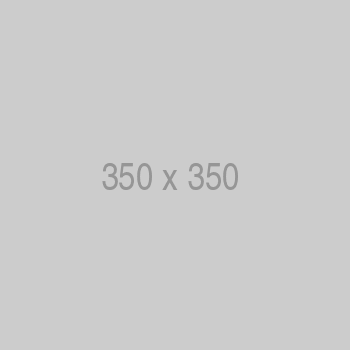
\includegraphics[width=0.3\linewidth]{images/placeholder.png}
  \caption{Visualisation des repères présents sur le système d'inspection par UGV.}
  \label{fig:ugv_frames}
\end{figure}

L'inspection se fait en 2 phases, l'exploration du périmètre (EP) présentée dans la section \ref{sec:perimeter_exploration} suivie de l'exploration des cavités (EC) présentée dans la section \ref{sec:cavity_exploration}. Dans la première phase, l'UGV fait le tour de la structure en sautant les cavités pour fermer la boucle le plus tôt possible. Ensuite, une analyse de la carte 3D est effectuée pour trouver les frontières indiquant des cavités non explorées dans la structure. Une trajectoire est planifiée pour diriger le robot vers la cavité pour cartographier l'intérieur de la structure. L'inspection se termine quand toutes les cavités ont été inspectées.

\begin{figure}[ht]
  \centering
  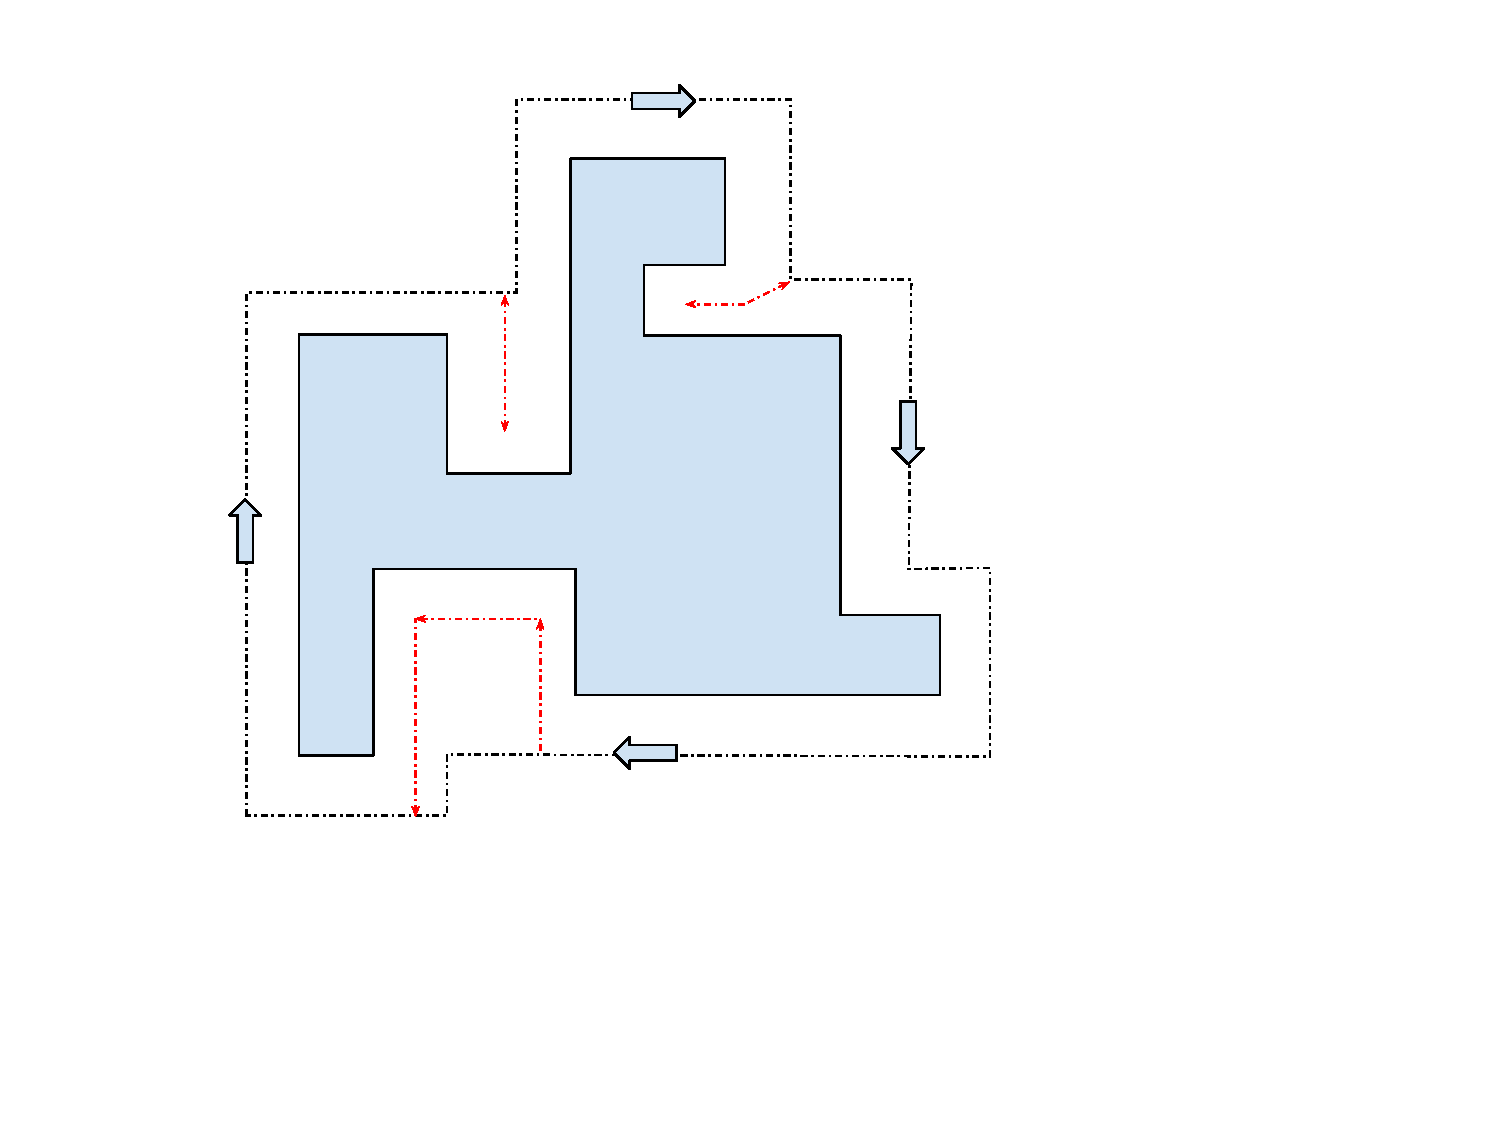
\includegraphics[width=0.5\linewidth]{images/ugv_goal}
  \caption{Illustration du but de l'algorithme. La périmètre trajectoire en noir indique l'exploration du périmètre qui saute les cavités pour revenir au point de départ le plus tôt possible et fermer la boucle. Les trajectoires rouges de la phase d'exploration de cavités viennent par après une fois que suffisamment de contraintes ont été mises sur la carte.}
  \label{fig:ugv_overview}
\end{figure}

\section{Exploration du périmètre} \label{sec:perimeter_exploration}

Suivant les hypothèses de la section \ref{sec:ugv_hypothesis}, le problème d'inspection se simplifie au parcours de la partie de la structure située entre les plans $z^g = 0$ et $z^g = H_{max}$. Pour ce faire la phase EP débute avec le robot près de l'un des murs de la structure. Le robot parcourt le périmètre dans le sens horaire gardant toujours une partie visible de la structure dans son champ de vision vers sa droite. À chaque itération de l'algorithme, l'UGV détermine la prochaine pose objectif auquel se rendre pour placer la caméra à une distance $D$ perpendiculairement à la surface de la structure, maximisant ainsi la qualité des détails perçus et la densité des points captés.

\subsection{Choix de la prochaine pose objectif}

L'algorithme \ref{alg:PE_next_goal} présente la méthode par laquelle nous calculons la prochaine pose objectif, permettant à l'UGV de suivre la surface de la structure. Étant donné un nuage de points $\mathca{P}$ provenant de la caméra, nous filtrons d'abord le sol en éliminant tous les points sous une certaine hauteur $z^g = s$. Ensuite à la ligne \ref{alg:slice:decoupe}, nous découpons $\mathca{P}$ pour obtenir un sous-ensemble $\mathca{S}$ adjacent à la prochaine section à inspecter, c'est-à-dire que $\mathca{S}$ est une partie (nous choisissons $1/3$) de $\mathca{P}$ vers la gauche de la caméra. Plus formellement, $\mathca{S}$ est choisi tel que les coordonnées en $y^c$ des points qui le composent satisfont
\begin{align}
  y^c_{max} - \frac{y^c_{max} - y^c_{min}}{3} \leq y^c \leq y^c_{max}
\end{align}
où $y^c_{max}$ et $y^c_{min}$ sont le maximum et le minimum des coordonnées $y^c$ de $\mathcal{P}$.

La \ref{alg:slice:pca}\textsuperscript{ième} étape est de déterminer la normale $\vect{n}$ de la surface. \citep{Rusu2009} explique que par le passé ceci aurait été fait en résolvant un problème des moindres carrés pour ajuster le modèle d'un plan $\Pi$ au nuage $\mathcal{S}$. On peut représenter le plan par un point $\vect{x}$ et un vecteur normal $\vect{n}$, et la distance d'un point $\vect{p}_i \in \mathcal{S}$ au plan est défini par $d_i = (\vect{p}_i - \vect{x} \cdot \vect{n})$. On choisi $\vect{x} = \vect{p}^c$ la moyenne des points de $\mathcal{S}$.
\begin{align}
  \vect{x} = \vect{p}^c = \frac{1}{k} \cdot \sum^{k}_{i=1} \vect{p}_i
\end{align}

Suivant une formulation par moindres carrés, on cherche donc à mettre les $d_i = 0$. La solution de $\vect{n}$ peut être trouvée par Analyse des Composantes Principales (ACP) en calculant les vecteurs propres et les valeurs propres de la matrice de covariance $\mathcal{C} \in \mathbb{R}^{3\times 3}$ de $\mathcal{S}$.
\begin{align}
  \mathcal{C} = \frac{1}{k} \sum^{k}_{i=1} (\vect{p}_i - \vect{p}^c) \cdot (\vect{p}_i - \vect{p}^c)^\top, \mathcal{C} \cdot \vect{v}_j = \lambda_j \cdot \vect{v}_j, j \in \{0, 1, 2\}
\end{align}
où $\mathcal{C}$ est semi-définie positive et les valeurs propres $\lambda_j \in \mathbb{R}^+$. Les vecteurs propres $\vect{v}_j$ forment ainsi une base orthonormale correspondant aux composantes principales de $\mathcal{S}$. En classant les valeurs propres par $0 \leq \lambda_3 \leq \lambda_2 \leq \lambda_1$, nous avons $\vect{v}_3$ le vecteur propre correspondant à la plus petite valeur propre $\lambda_3$ qui est donc une approximation de la normale $\pm \vect{n} \sim \vect{v}_{3}$ du plan $\Pi$, mais avec une ambiguïté de signe.

\begin{algorithm}[ht]
  \SetAlgoLined
  \SetKwData{Left}{left}\SetKwData{This}{this}\SetKwData{Up}{up}
  \SetKwFunction{Union}{Union}\SetKwFunction{FindCompress}{FindCompress}
  \SetKwInOut{Input}{entrée}\SetKwInOut{Output}{sortie}
  \Input{$\mathcal P$ Le nuage de point provenant de la caméra}
  \Input{$D$ La distance à garder par rapport aux murs}
  \Output{${po}$ la position objectif de la caméra}
  \Output{$\vect{u}$ le vecteur d'orientation de la caméra}

  $\mathcal S$  $\gets$ FiltrageDuSol($\mathcal P$)   \\
  $\mathcal S$  $\gets$ DécoupeAvant($\mathcal S$) \label{alg:slice:decoupe}   \\
  $\vect{p}^c$         $\gets$ Moyenne($\mathcal S$)         \\
  $[\vect{v}_1, \vect{v}_2, \vect{v}_3; \lambda_1, \lambda_2, \lambda_3] \gets$ AnalyseComposantesPrincipales($\mathcal S$) \label{alg:slice:pca}\\
  $\vect{\tilde u} \gets \vect{v}_3 - (\vect{v}_3\cdot\vect{z}_{\fr c})\vect{v}_3 $ \tcp*[r]{Projection vers le plan $\vect{x_c}\vect{y_c}$} \\
  $\vect{u} \gets \vect{\tilde u} \; \text{sign}(\vect{\tilde u} \cdot \overrightarrow{O_{\fr c} \overline{p}^{\fr c}}); \vect{u} \gets \vect{u}/\|\vect{u}\|$ \label{alg:slice:sign} \\
  $\vect{r} \gets \vect{z}_{\fr c} \times \vect{u}$ \\
  \tcp{Vérification de la largeur de $\mathcal{S}$}
  \eIf{$y^c_{max} - y^c_{min} > w$­­­­}{
    $\alpha = \frac{y^c_{max} - y^c_{min}}{6}$ \tcp*[r]{Calcul de la longueur de pas à prendre}\\
    ${po^c} \gets p^c - D \vect{u} + \alpha \vect{r}$   \label{alg:slice:po} \\
  }{
    ${po^c} \gets p^c + D \vect{r}$
  }
  \Return ${po^c}, \vect{u}$

  \caption{Calcul de la prochaine pose objectif au moyen du nuage de point courant de la caméra.}
  \label{alg:PE_next_goal}
\end{algorithm}

Le vecteur normal $\vect{v}_3$ est projeté sur le plan $\vect{x}_c\vect{y}_c$ sur lequel repose la caméra et pour résoudre l'ambiguïté de signe possible provenant de $\vect{v}_3$, $\vect{u}$ est pris pour pointer dans la direction du vecteur $\overrightarrow{O_{\fr c} \overline{p}^{\fr c}}$, c'est-à-dire de la caméra au centre de $\mathcal{S}$. L'algorithme retourne aussi la position objectif ${po}$ de la caméra, calculé à partir de $-D\vect{u}$ pour garder la bonne distance au mur et $\alpha \vect{r}$ pour faire avancer le robot autour des coins de la structure. La Figure \ref{fig:ugv_goal_determination} permet de mieux visualiser cet effet; $\vect{r}$ repose sur le plan $\Pi$ et permet à la caméra de voir autour des coins pour passer au prochain mur à inspecter. Une limite à cette approche est que dans le cas de coins aigus ou de murs particulièrement minces, la caméra ne pourra avancer assez pour voir la suite du mur. Nous pouvons détecter ce cas quand la largeur de $\mathcal{S}$ tombe en dessous d'un certain seuil $w$; c'est à ce moment que ${po}$ est calculé par ${po} \gets p^c + D \vect{r}$, forçant ainsi l'UGV à tourner autour du coin.

Finalement ${po^c}$ est transformé dans le repère $\mathsf{G}$ pour fins de navigation. Le but du robot devient donc de bouger de façon à placer $O_c$ à ${po^g}$ et d'orienter la caméra selon $\vect{u}$.

\begin{figure}[ht]
  \centering
  \subfloat[]{
  	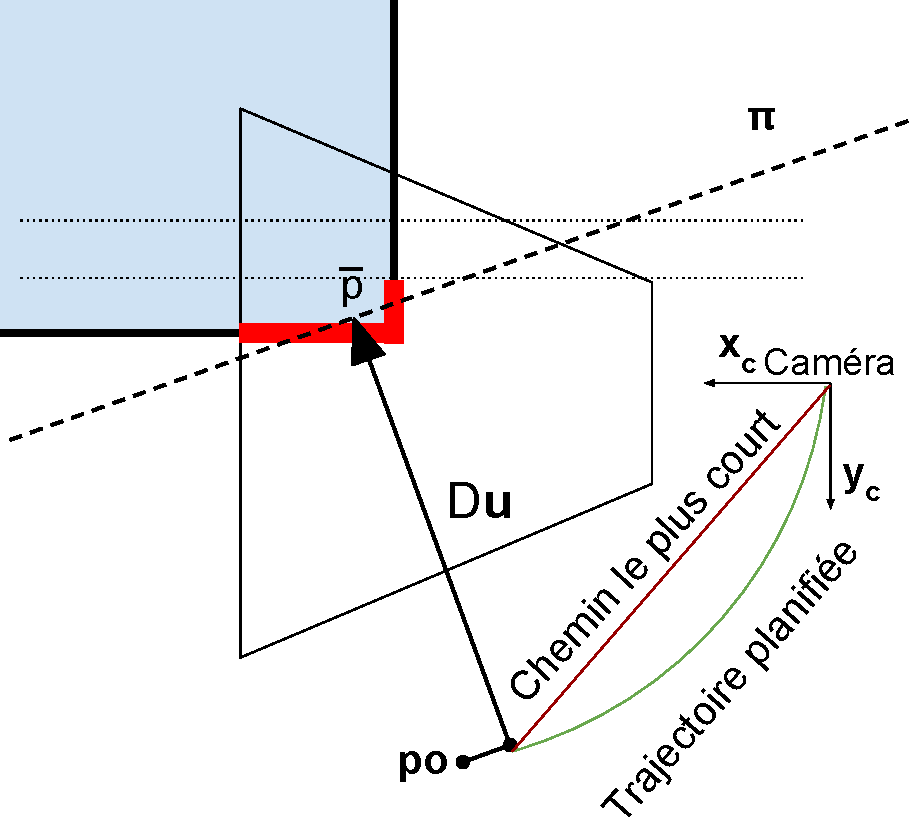
\includegraphics[width=0.45\linewidth]{images/nbv}
  	\label{subfig:ugv_nbv}
  }
  \hfil
  \subfloat[]{
  	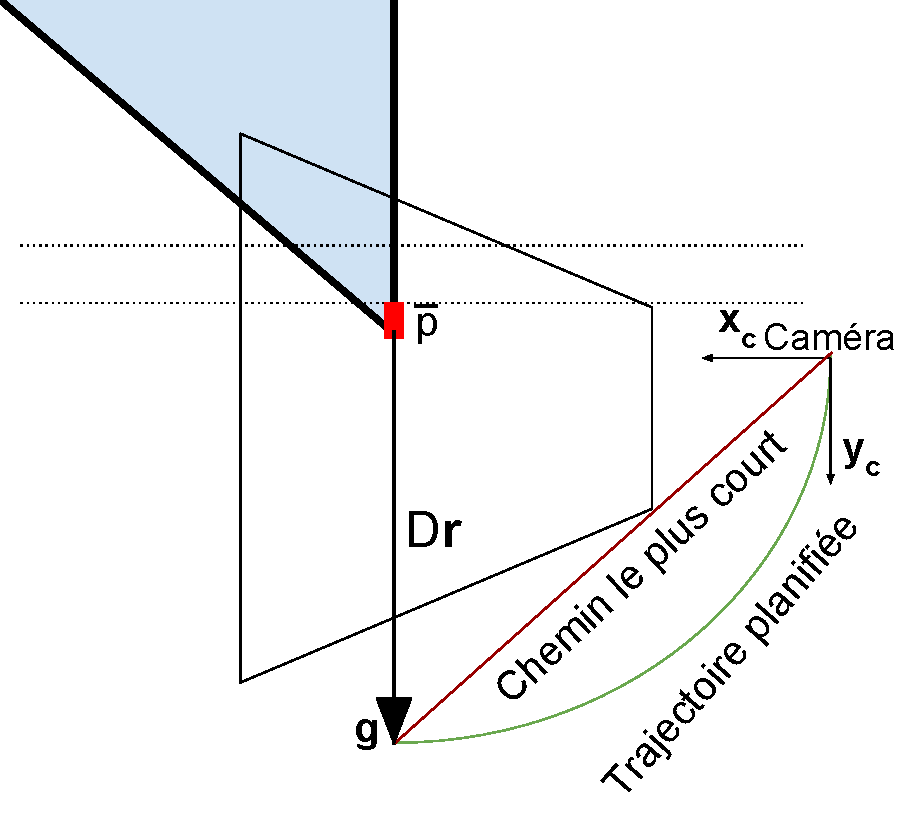
\includegraphics[width=0.45\linewidth]{images/nbv_acute}
  	\label{subfig:ugv_acute_angle}
  }
  \caption{
    Illustration du calcul de la prochaine pose objectif autour d'un coin a) dans le cas normal b) dans le cas d'un coin à angle aigu.
  }
  \label{fig:ugv_goal_determination}
\end{figure}

\subsection{Planification de trajectoire locale}

Puisque notre robot est terrestre, la tâche de planification de trajectoire se simplifie en deux dimensions. Pour ce faire, le modèle 3D en construction est projeté sur une grille 2D pour établir une carte d'occupation. On prend un sous-ensemble local de la carte de taille $2D \times 2D$ (nous rappelons que $D$ est la distance à la structure désirée) autour de la position de la caméra pour calculer une trajectoire par champ de potentiel \citep{Khatib1990, Choset2005}. Soit $k$ cellules occupées aux coordonnées $\{x_j\}^k_{j=1}$, nous avons la fonction de potentiel
\begin{align}
  N(x) &= \alpha \| x - {po}^g \|^2 + \sum^k_{j=1} I_j(x)d_j(x)
\end{align}
où $\alpha$ est un scalaire. La fonction de répulsion $d_j$ définie par:
\begin{align}
  d_j &= \frac{1}{\beta \| x - x_j \|}
\end{align}
où $\beta$ est un scalaire et $I_j(x)$ est le terme limitant la portée de $d_j$ par
\begin{align}
  I_j(x) =     \begin{cases}
      1, & \text{si}\ \|x - x_j\| \leq D \\
      0, & \text{autrement}
    \end{cases}
\end{align}
Pour guider le robot à sa destination, il suffit de suivre le gradient négatif du champ de potentiel en envoyant des commandes de vitesses à l'UGV, i.e. $\dot x = -\nabla N(x)$ avec
\begin{align}
  - \nabla N(x) = 2 \alpha ({po}^g - x) + \sum_{i \in J_x}\frac{1}{\beta \| x - x_i\|^3}(x - x_i)
  \label{eq:ugv_potential_field_gradient}
\end{align}
où $J_x = \{ j : I_j(x) = 1\}$ l'ensemble des cellules occupées de la carte dans un voisinage $D$ de $x$.

En d'autres mots, considérons $\mathcal M_D = \left\lbrace x : J_{x} \neq \emptyset \right\rbrace $ la région à l'intérieur d'une distance $D$ de la structure, pour une petite valeur de $\beta$ le terme de répulsion dans l'équation \ref{eq:ugv_potential_field_gradient} repousse le véhicule. Quand l'UGV se situe en dehors de $\mathcal M_D$, le premier terme de l'équation \ref{eq:ugv_potential_field_gradient} devient dominant et attire le véhicule vers $po^g$. Nous arrêtons de suivre le gradient une fois que l'UGV se retrouve dans un certain rayon d'acceptation de la position objectif, après quoi nous recommençons l'algorithme \ref{alg:PE_next_goal}.

\begin{figure}[ht]
  \centering
  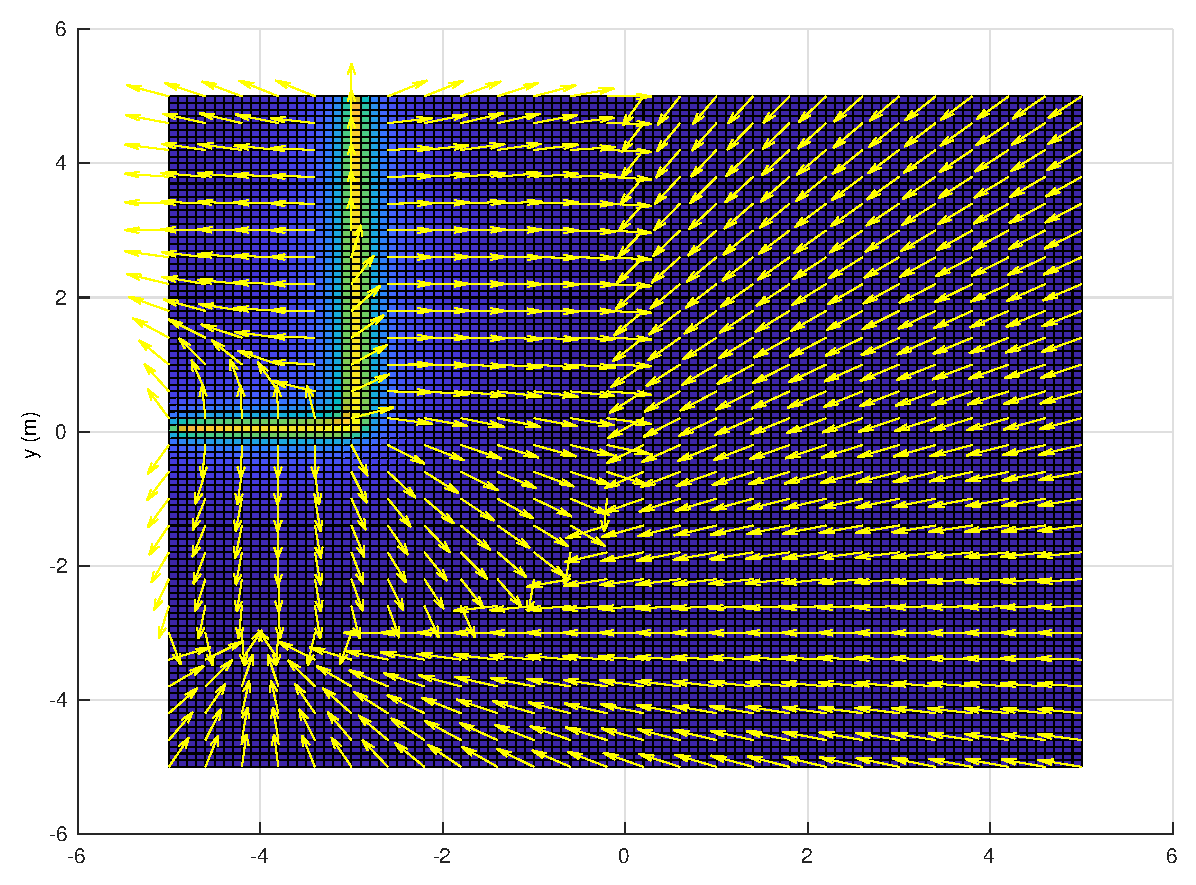
\includegraphics[width=0.7\linewidth]{images/champ_de_potentiel.eps}
  \caption{Exemple de visualisation du champ de potentiel. Les carrés jaunes représentent un mur et les vecteurs représentent la direction du gradient. }
  \label{fig:potential_field}
\end{figure}

En somme, les équations et les algorithmes ci-dessus permettent au robot parcourir incrémentalement la surface de la structure en gardant un point de vue orthogonal aux murs.

\subsection{Saut de cavités}
\label{subsec:ugv_cavity_skip}

Prenons maintenant l'exemple de la Figure \ref{fig:ugv_exploration}, alors que le robot s'apprête à tourner autour du coin pour entrer dans la cavité. Le détecteur d'obstacles se déclenche en voyant le mur arrière. D'une part, nous voulons éviter d'entrer dans la cavité et d'autre part nous voulons empêcher le robot de s'approcher à moins d'une distance $D$ d'un mur qui se retrouverait hors de son champ de vision. C'est pourquoi lorsque l'obstacle est détecté, le robot s'arrête et tourne le capteur de profondeur dans la direction de la détection. L'algorithme \ref{alg:PE_next_goal} est réexécuté avec le nouveau nuage de points $S$ pris en avant du robot et la trajectoire d'inspection se poursuit vers la gauche.

\begin{figure}[ht]
\centering
\subfloat[]{
	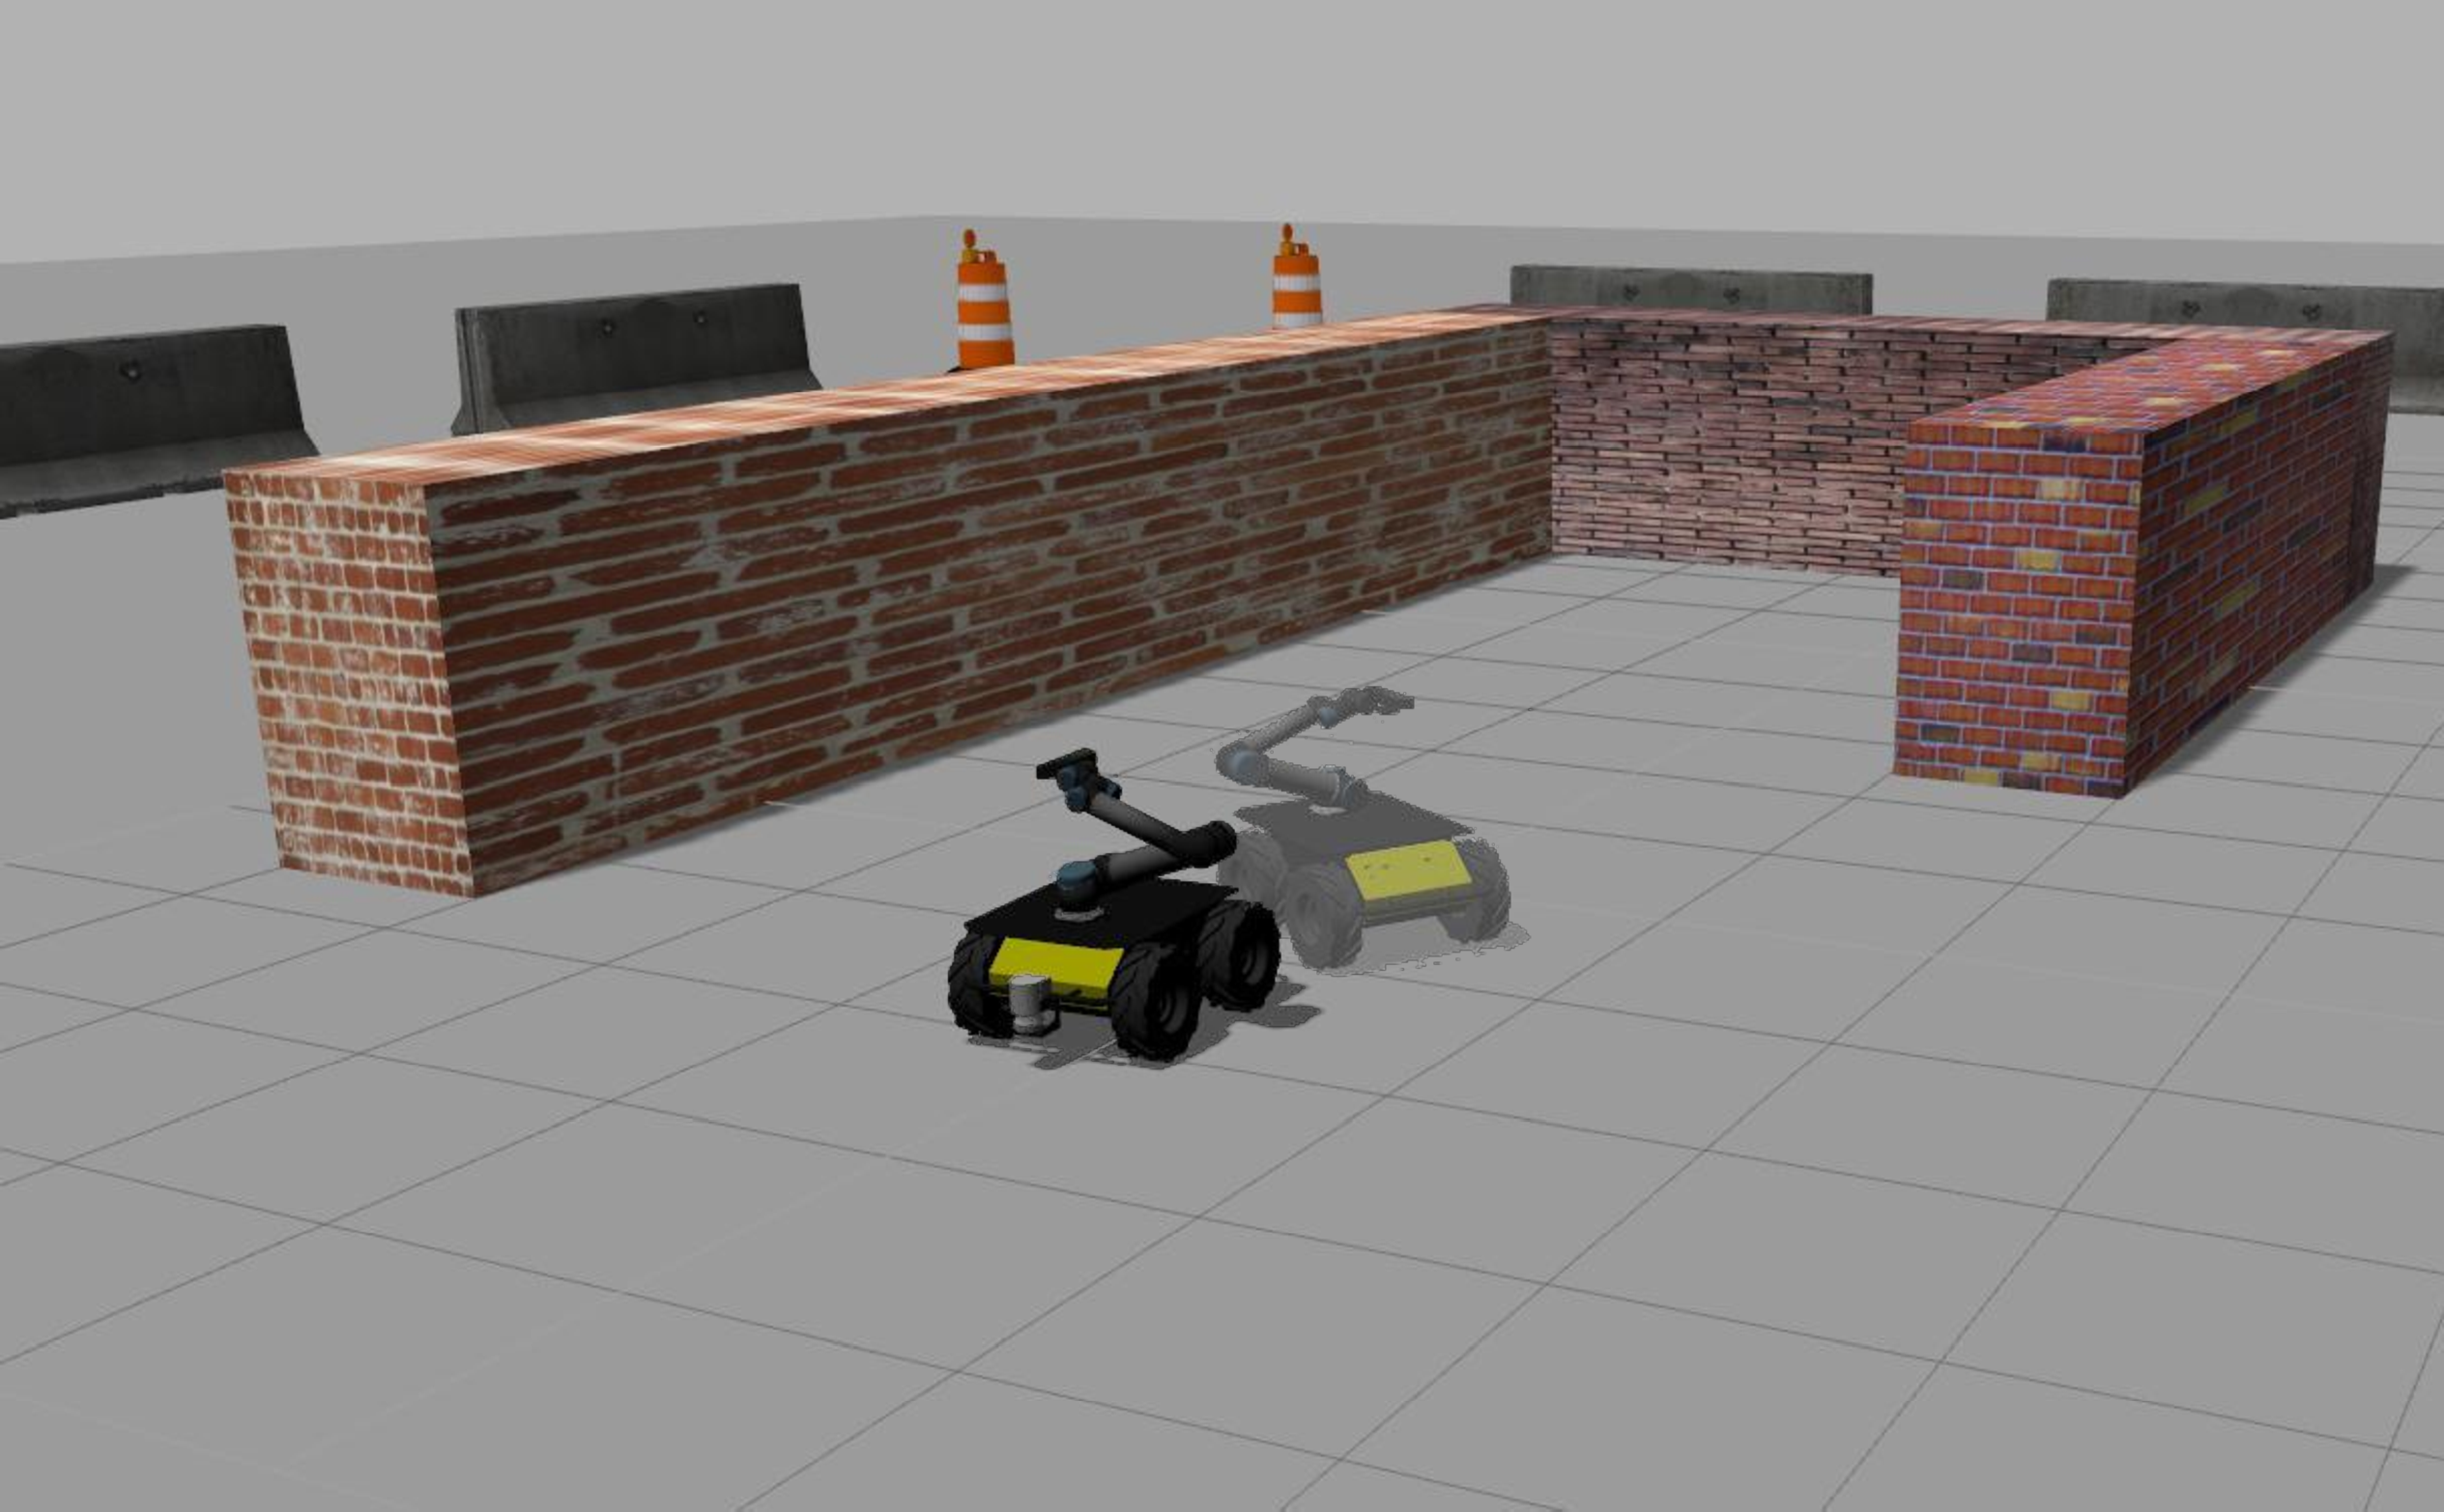
\includegraphics[width=0.45\linewidth]{images/Lookahead}
	\label{subfig:ugv_gazebo}
}
\hfil
\subfloat[]{
	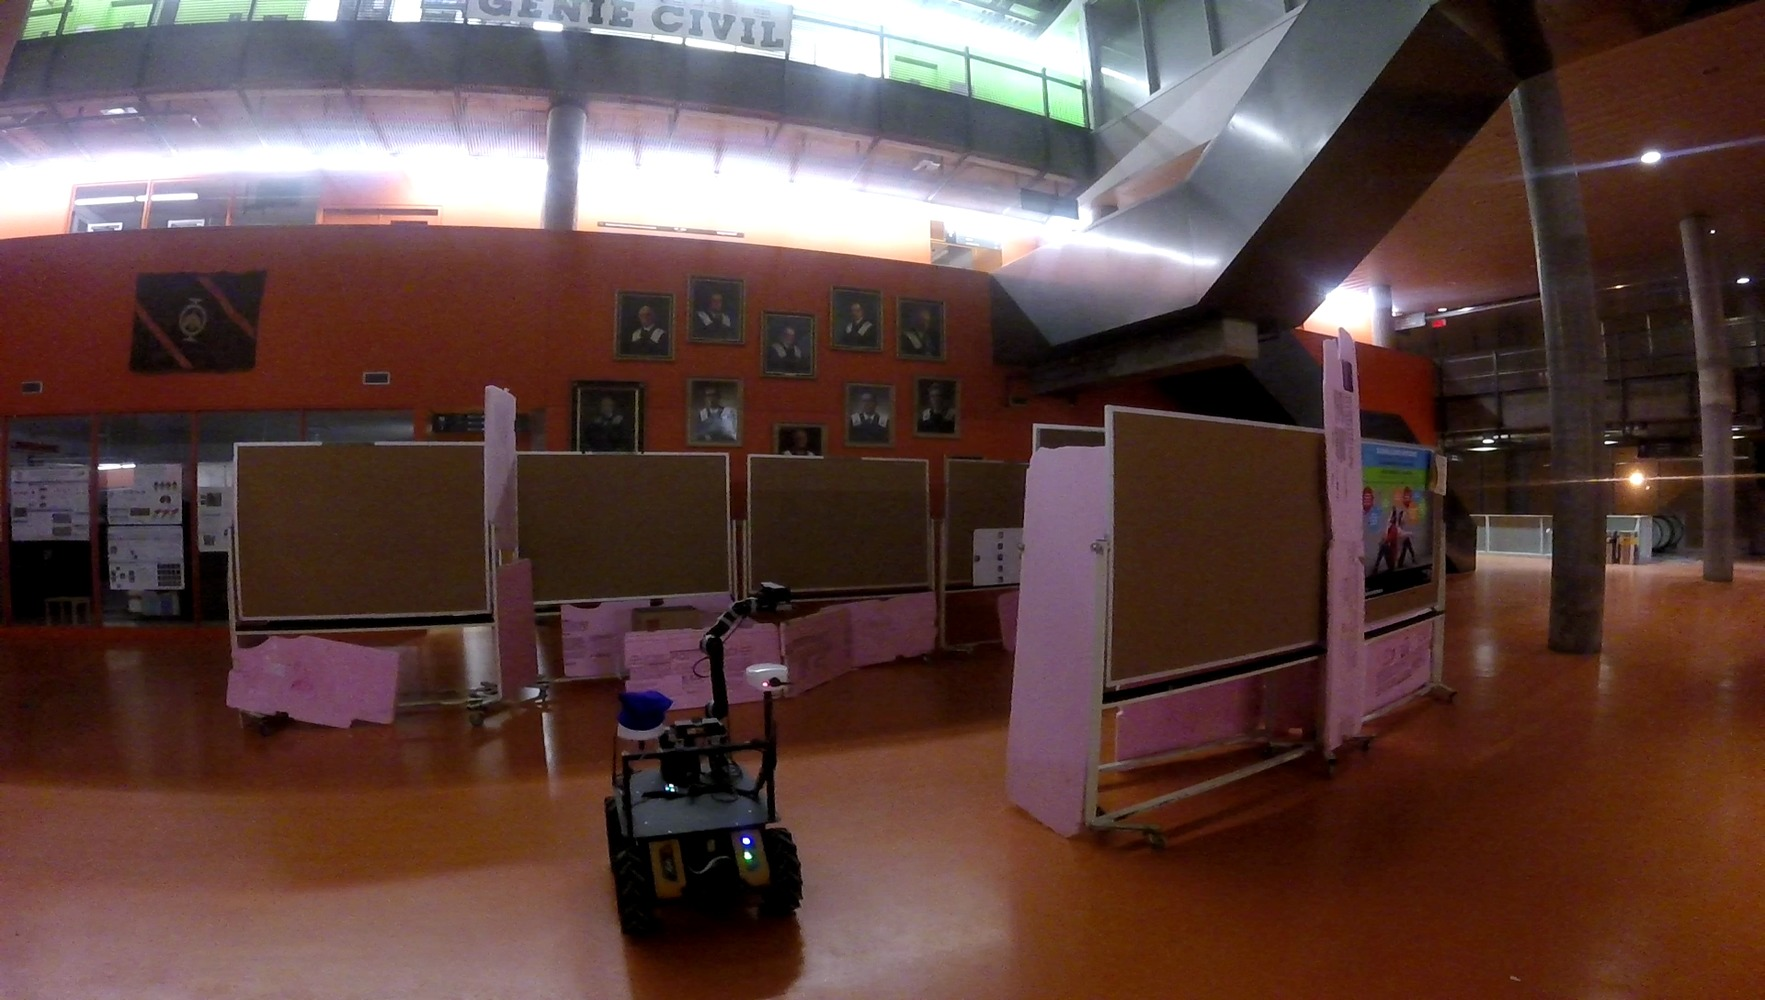
\includegraphics[width=0.45\linewidth]{images/ugv_interference.jpg}
	\label{subfig:ugv_interference}
}
\caption{
Exemple de détection d'obstacle et de saut de cavité. a) Le robot (transparent) tente de tourner autour du coin, mais détecte un mur vers l'avant. La trajectoire est replanifiée pour continuer vers la gauche sans entrer dans la cavité.}
\label{fig:ugv_exploration}
\end{figure}

\subsection{Fin de l'exploration de périmètre}

La phase EP se termine lorsqu'une fermeture de boucle globale est détectée par le module de SLAM. Ceci peut être difficile si la trajectoire a accumulé trop d'erreurs ou si l'environnement ne comporte pas de caractéristiques uniques permettant au système de SLAM de définitivement détecter le retour à un endroit connu. C'est pourquoi nous recommandons l'ajout d'un objet unique à la position de départ du robot pour assurer une bonne fermeture de boucle. Dans nos tests, ceci consistait en une pancarte colorée placée sur la surface de la structure telle que dans la Figure \ref{fig:ugv_pancarte}.

\begin{figure}[ht]
  \centering
  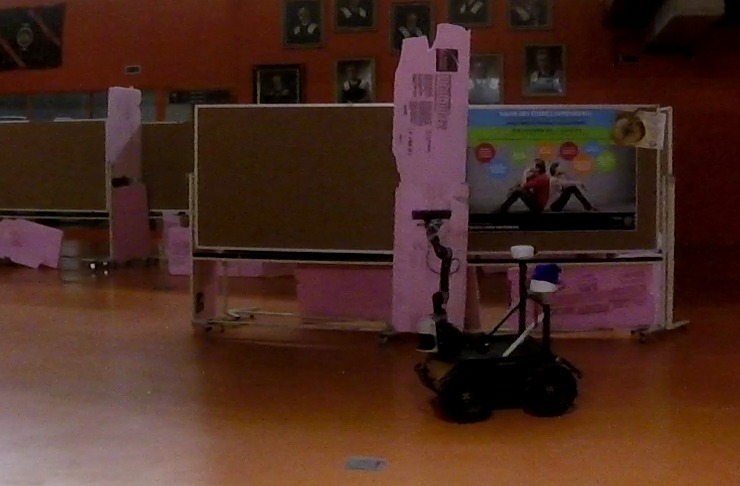
\includegraphics[width=0.5\linewidth]{images/ugv_unique.jpg}
  \caption{Exemple d'objet unique à placer au point de départ pour assurer une fermeture de boucle.}
  \label{fig:ugv_pancarte}
\end{figure}

\section{Finition du modèle} \label{sec:cavity_exploration}

Au terme de la phase EP, le modèle de la structure produit par le module de SLAM demeure incomplet pour deux raisons possibles. La première est due à des occlusions présentes dans les régions explorées provenant de la structure elle-même par sa forme irrégulière ou par un échec du capteur de profondeur. La deuxième provient des régions non explorées qui ont été ignorées par la phase EP par la man\oe uvre expliquée à la section \ref{subsec:ugv_cavity_skip}. Dans cette section, nous profitons du deuxième cas pour détecter les régions qui restent à explorer nous permettant ainsi compléter le modèle.

\subsection{Détection des cavités}

À mesure que la robot cartographie la structure, la séquence de nuages de points est rassemblée dans un grand modèle contenant tous les nuages que le module de SLAM considère comme utiles à intégrer. Suite à la fermeture de la boucle, nous avons une estimation optimale de toutes les poses du robot à partir desquelles chaque nuage de points a été capté. Grâce à cette information, il est possible d'effectuer un traçage de rayon dans une OctoMap \citep{Hornung2013} pour nous donner une représentation 3D de l'environnement qui inclut les espaces vide, occupé et inconnu.

Suivant la définition posée par \citep{Yamauchi1997}, un voxel frontière (\emph{frontier}) est voxel non occupé adjacent à un voxel de l'espace inconnu. Grâce à notre OctoMap, il est donc possible de calculer l'ensemble de tous les voxels frontières. Une particularité de l'utilisation d'une caméra de profondeur lors de l'inspection est que l'espace connu prend la forme d'un tronc de pyramide correspondant au champ de vision de la lentille. Ceci a pour effet, tel que l'on peut voir dans la Figure \ref{subfig:ugv_frontier} que la carte finale inclut une grande quantité de voxels frontières correspondant aux hauts et aux bas des troncs de vue utilisés pour construire la carte.

\begin{figure}[!h]
  \centering
  \subfloat[]{
  	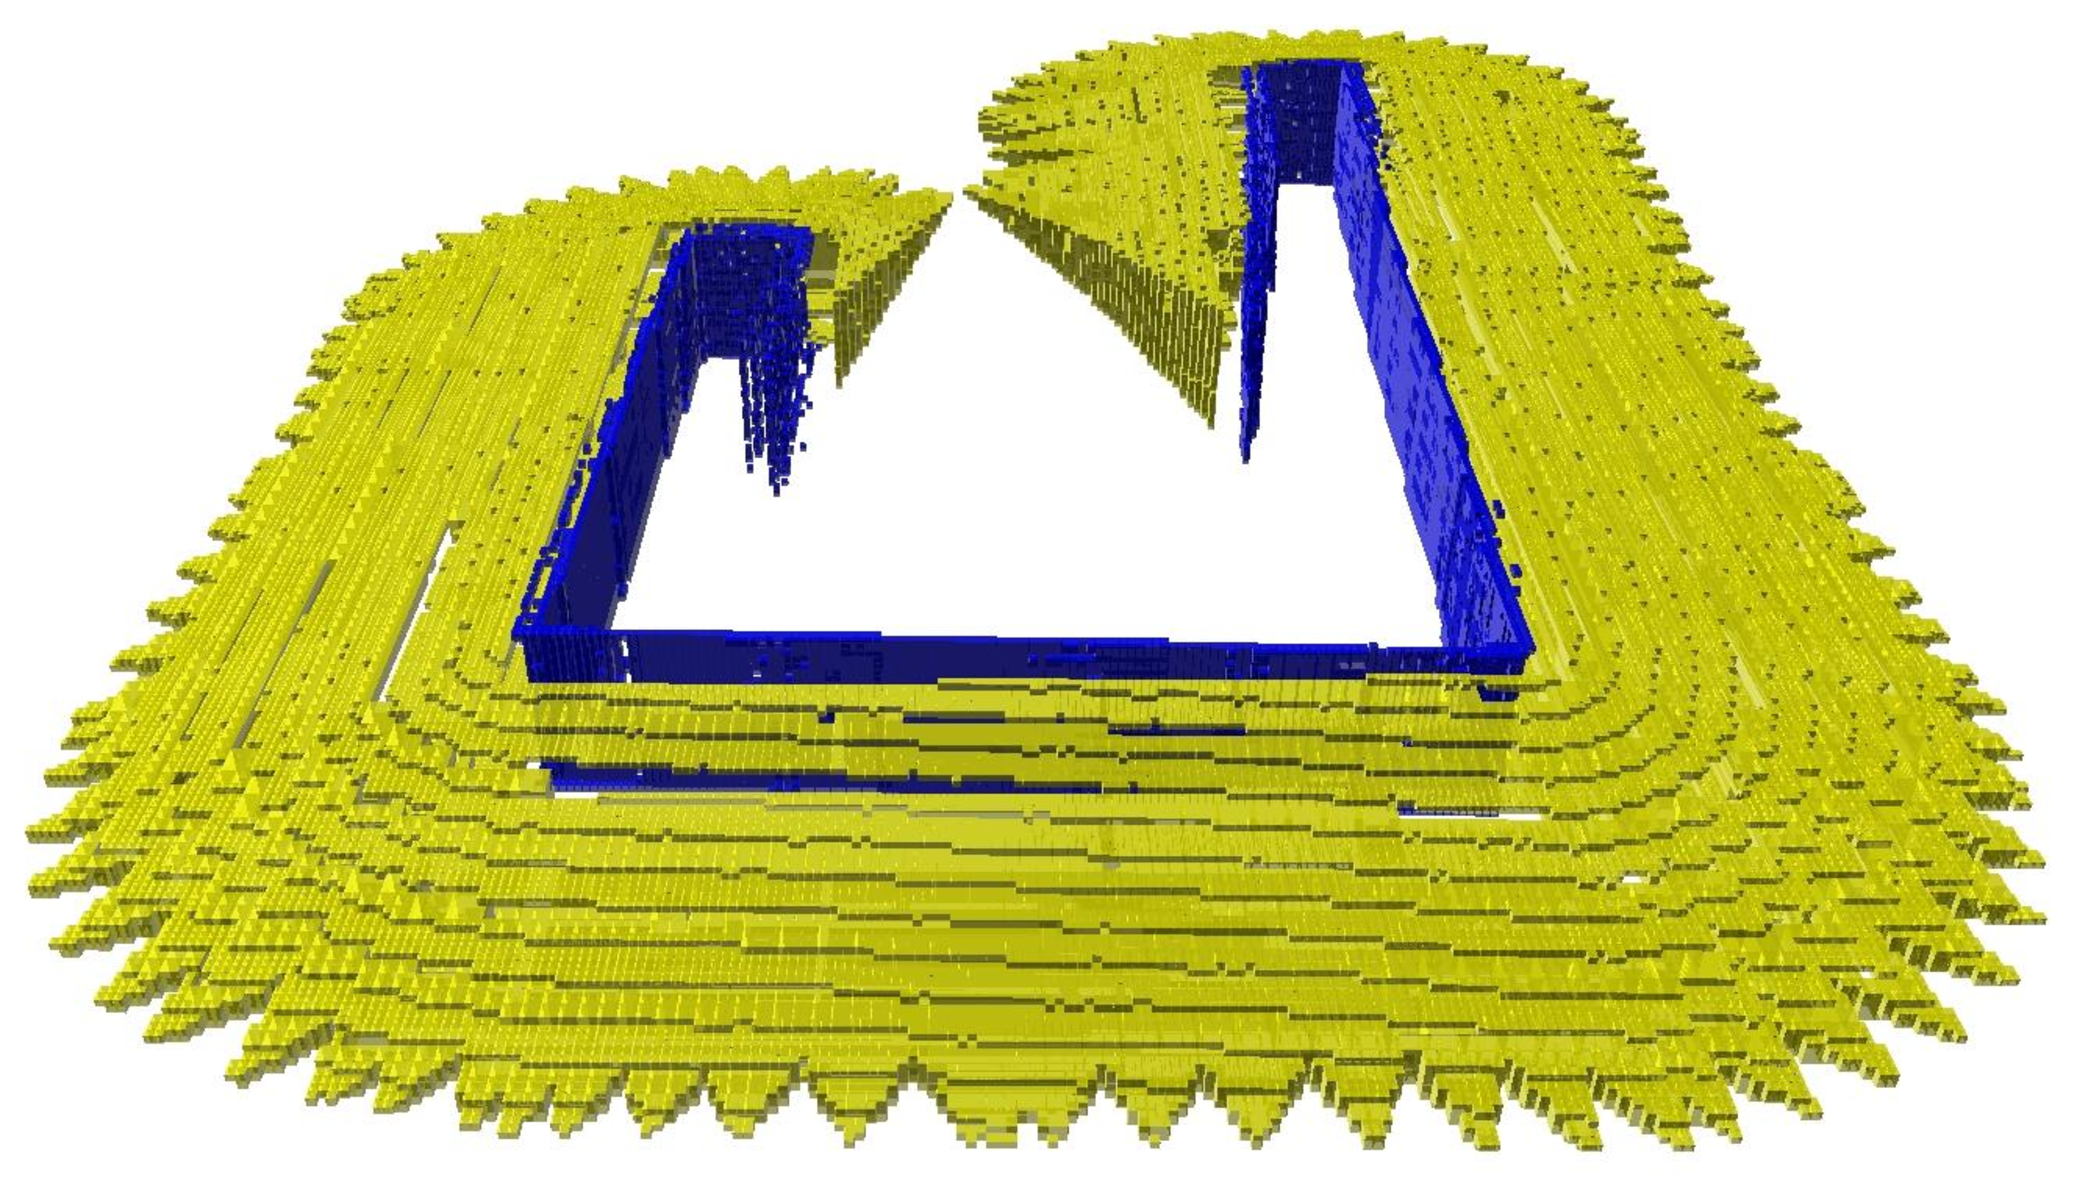
\includegraphics[width=0.45\linewidth]{images/frontier_candidates}
  	\label{subfig:ugv_frontier}
  }
  \hfil
  \subfloat[]{
  	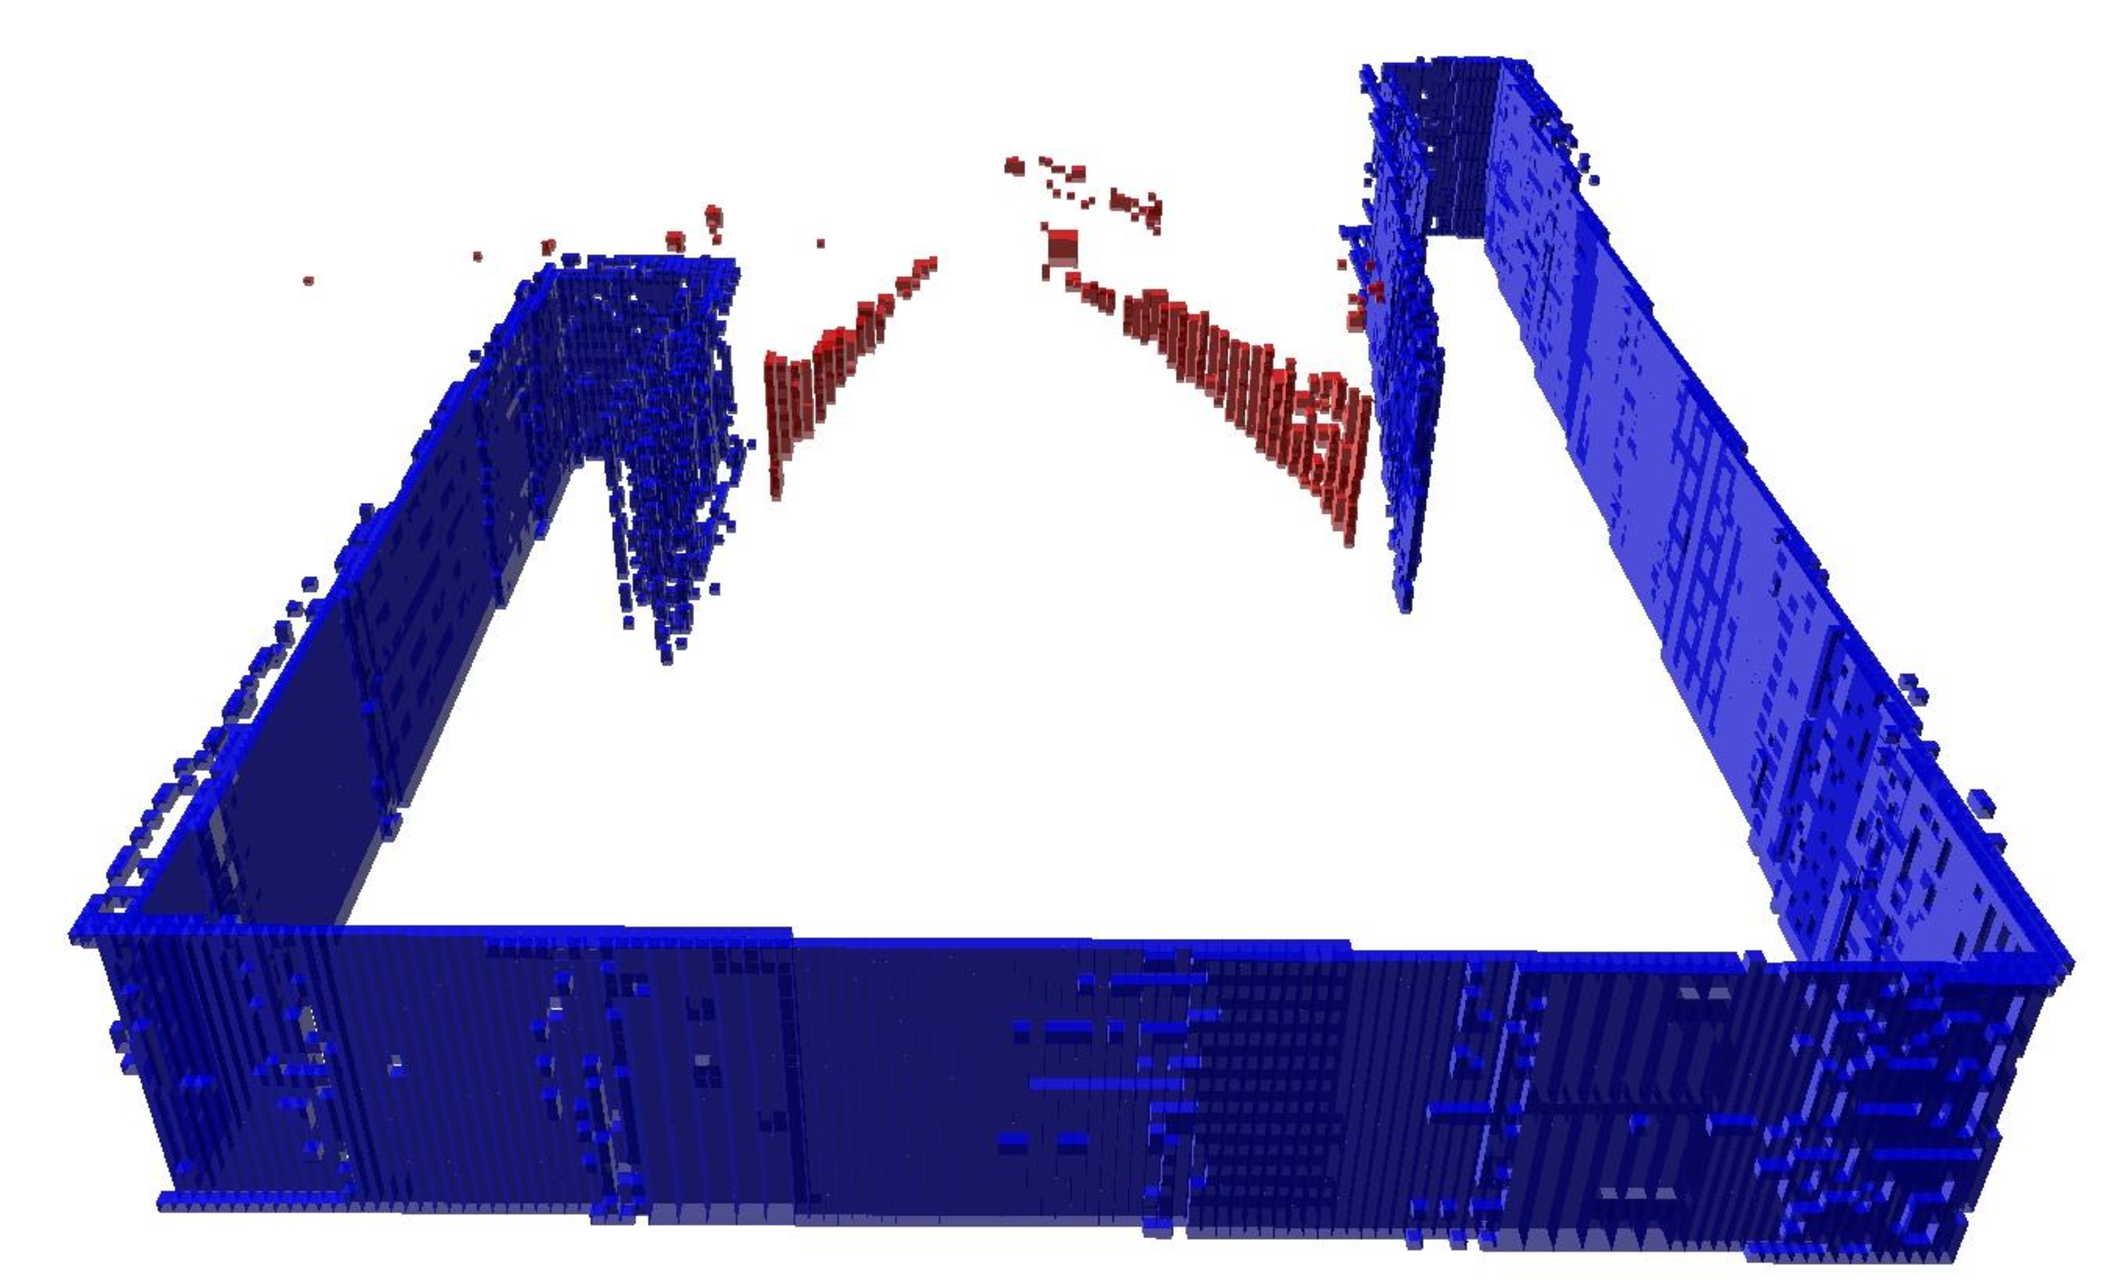
\includegraphics[width=0.45\linewidth]{images/frontier_voxels}
  	\label{subfig:ugv_entrance}
  }
  \caption{
    Analyse de la OctoMap avant le début de la phase d'exploration de cavités.
    a) En jaune les voxels frontières et en bleu les voxels faisant partie de la structure.
    b) En rouge les voxels frontières identifiant une entrée de cavité.
  }
  \label{fig:ugv_frontier}
\end{figure}

\begin{algorithm}[!ht]
  \SetAlgoLined
  \SetKwData{Left}{left}\SetKwData{This}{this}\SetKwData{Up}{up}
  \SetKwFunction{Union}{Union}\SetKwFunction{FindCompress}{FindCompress}
  \SetKwInOut{Input}{entrée}\SetKwInOut{Output}{sortie}

  \Input{$\mathcal G$ Le graphe des poses optimisées de la carte et les nuages de points associés}
  \Output{$\mathcal F$ L'ensemble des voxels frontières}

  \ForEach{$nuage^c$, $pose^g$ $\in \mathcal G$}{
    %Transform $p^c$ to $p^g$\\
    $nuage^g \gets T^g_c {nuage}^c$\\
    $nuage^g \gets $ SeuillageDuSol($nuage^g$)\\
    $nuage^g \gets $ SeuillageDuPlafond($nuage^g$)\\
    Insertion et traçage de rayon de $nuage^g$ dans l'OctoMap\\
  }\\

  %cloudmap_cb\\
  %  \Indp
  %  remove ground plane\\
  %  constrain bounding box of octomap using full map\\
  %  reconstruct convex hull\\
  %  \Indm
  %determine frontiers\\
  %  \Indp
    \ForEach{voxel $\in$ OctoMap}{
      \If{voxel.estVide() $\&\&$ 6-connexité inclut au moins un voxel d'espace inconnu}{
        Ajouter le voxel à l'ensemble des frontières candidates $\mathcal C$
      }
    }\\
    %crop out candidates outside of hull\\
    \ForEach{c $\in \mathcal C$}{
      $v \coloneqq $ L'ensemble des voxels dans un voisinage $k$ de $c$\\
      $\vec{n}_i^g \gets $ ACP($v$) \tcp*[r]{Estimation de la normale par ACP}\\
      \If{$| {\vec{n}_i}_z^g | < \alpha \ \&\& $ voisinage $d_0$ de $c$ n'est pas occupé }{
        Ajouter $c$ à $\mathcal F$\\
      }\\
    }\\
  %  \Indm
  \Return $\mathcal F$

  \caption{Recherche de voxels frontières indiquant une entrée de cavité possible dans la OctoMap.}
  \label{alg:CE_detection}
\end{algorithm}

Suivant l'algorithme \ref{alg:CE_detection}, nous pouvons filtrer les voxels frontières selon la normale de la surface composée des voxels dans un certain voisinage $k$ du voxel considéré. Si $| n_z^g | < \alpha$ pour une certaine tolérance $\alpha$ le voxel est gardé. Une deuxième passe est réalisée pour enlever les frontières trop proches de la structure; ceci permet d'éliminer les défauts provenant d'occlusions ou d'échecs de perception. Le seuil $d_0$ utilisé peut être choisi par une fraction de la distance de sécurité, par exemple $d_0 = 0.1D$. Le résultat final de l'algorithme \ref{alg:CE_detection} appliqué à l'OctoMap présentée dans la Figure \ref{subfig:ugv_frontier} est visible dans la Figure \ref{subfig:ugv_entrance}.

Nous avons maintenant un ensemble de voxels faisant possiblement partie des entrées de cavités dans la structure. Ces voxels sont partitionnés par leur distance euclidienne selon un algorithme de remplissage par diffusion. Les partitions dont la surface est en dessous d'un certain seuil sont supprimées. Ce seuil peut être déterminé intuitivement par exemple en fonction de $D$ et de la largeur du robot. Nous pourrions par exemple supprimer toute entrée ne donnant pas assez d'espace au robot pour man{\oe}uvrer. À la fin de cette procédure, chaque partition représente une entrée de cavité.

\subsection{Exploration des cavités}

\begin{figure}[ht]
  \centering
  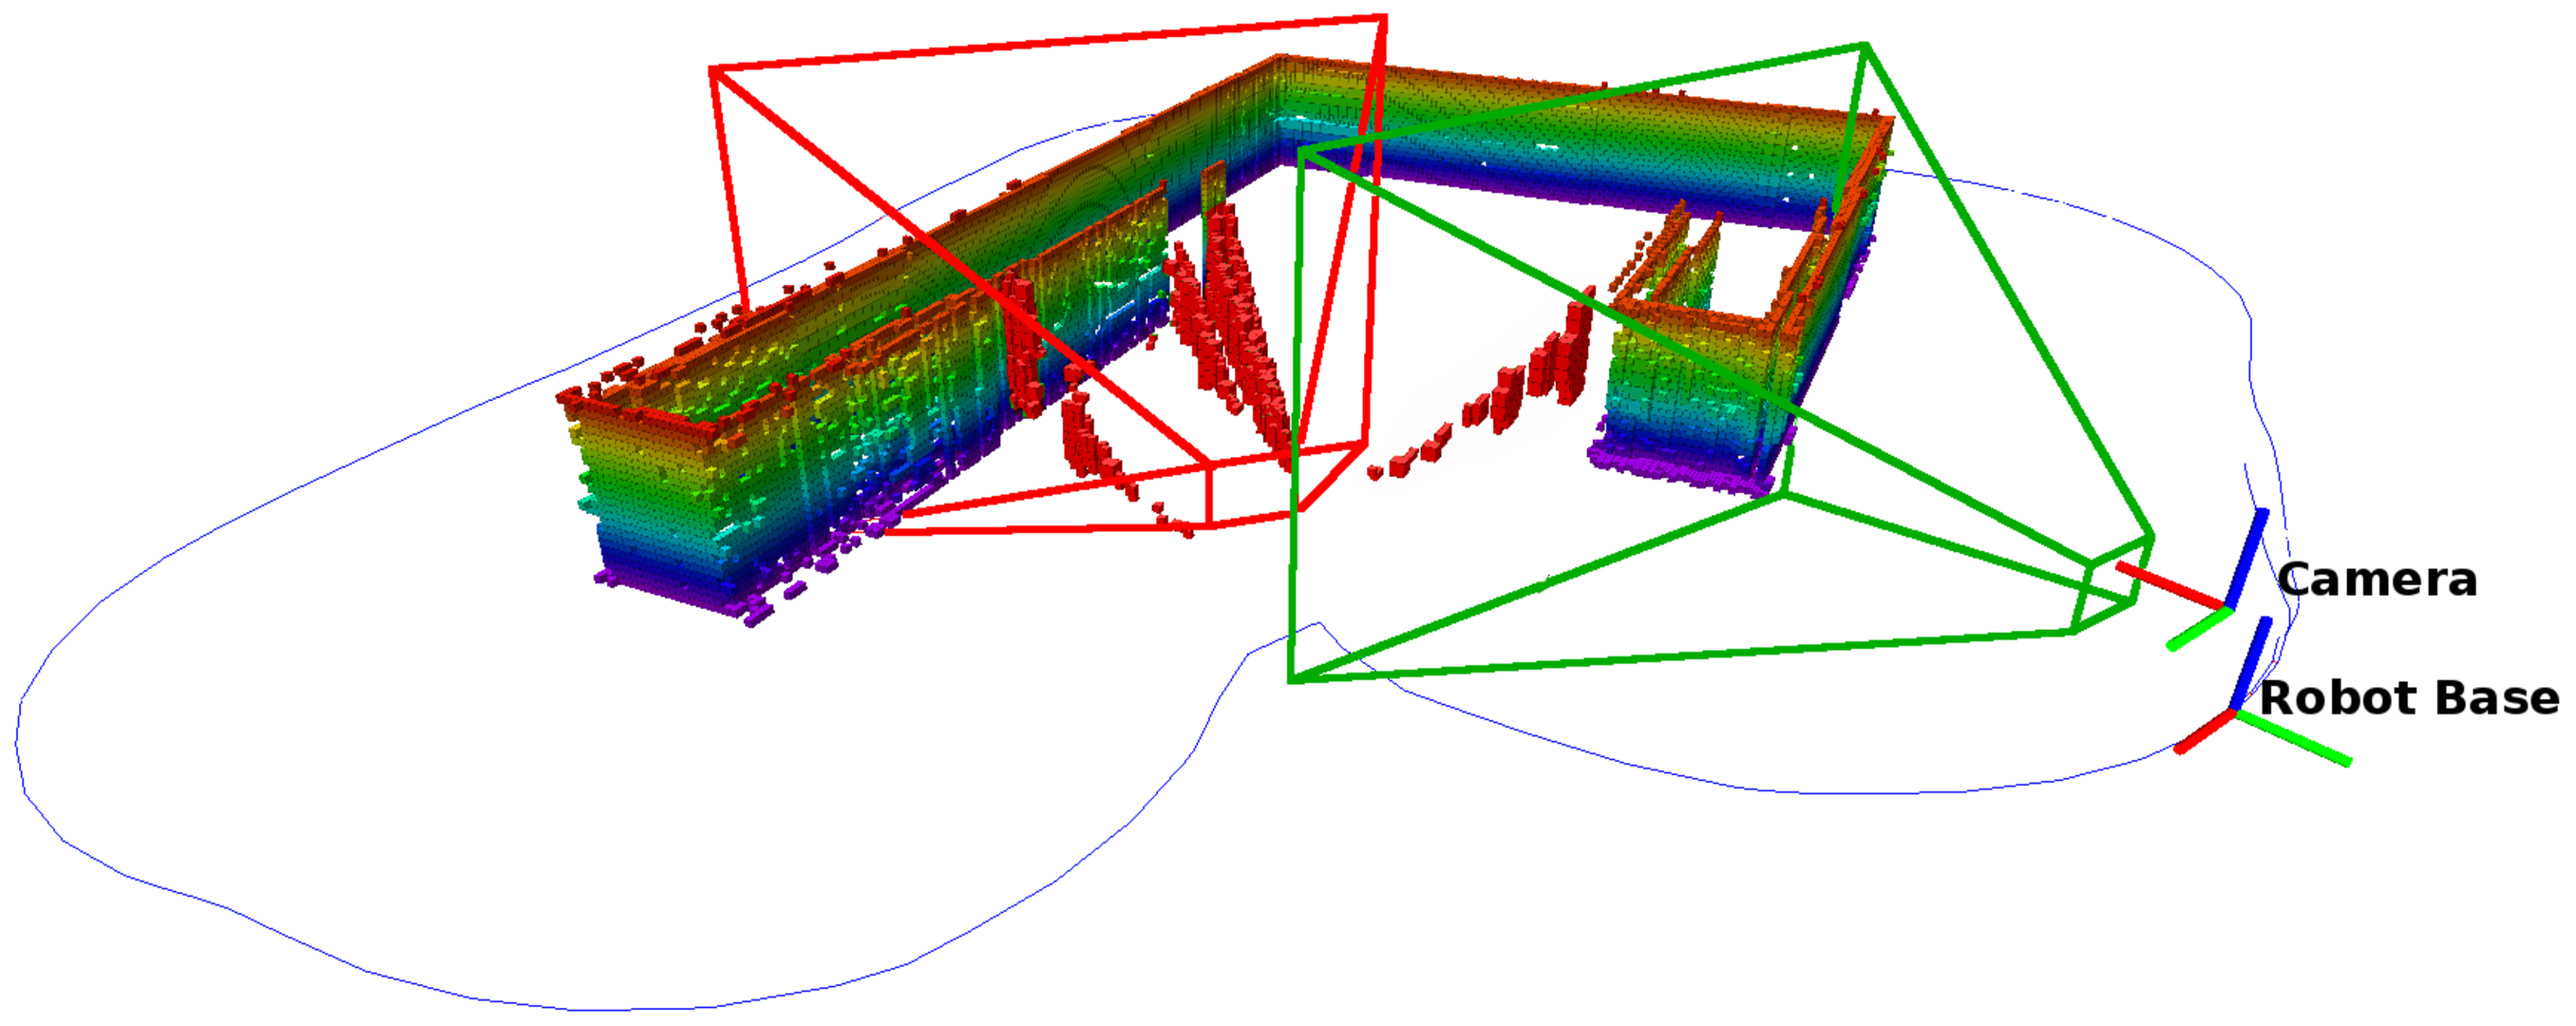
\includegraphics[width=0.8\linewidth]{images/CE_start}
  \caption{Début de la phase EC avec les points de vue associés à chaque entrée détectée.}
  \label{ugv:debut_ec}
\end{figure}

Une fois les entrées de cavités trouvées, il est possible de commencer la phase d'exploration des cavités (EC). Pour ce faire, chaque cavité est explorée de façon similaire à la phase EP, c'est-à-dire par suivit de mur en gardant la caméra orthogonale à la surface, mais cette fois-ci à une distance $\Delta \in [\delta, D]$ où $\delta$ est la distance de perception minimale. Nous verrons plus tard comment choisir $\Delta$, mais avant nous devons examiner la façon de choisir un point de vue (PDV) de départ pour débuter la phase EC.

En ordonnant les poses du graphe $\mathcal G$ provenant du système de SLAM par horodatage, nous choisissons pour chaque entrée la première pose qui possède une vue non obstruée au centroïde des voxels composant l'entrée. Cette liste de poses objectifs est à son tour ordonnée par horodatage et explorée en ordre. Comme nous pouvons l'observer dans la Figure \ref{ugv:debut_ec}, la détection d'entrée calculera typiquement deux entrées par cavité, parfois plus. Ceci provient du fait qu’une grande cavité aura des voxels frontières de part et d'autre de l'entrée tel que l'on peut voir dans la Figure \ref{subfig:ugv_entrance}.  Pour éviter la redondance dans la phase EC, si le centroïde d'une entrée entre en vue lors de l'exploration, l'entrée est enlevée de la liste.

La phase EC requiert une méthode de navigation légèrement différente de la phase EP. Premièrement, la détection d'obstacles se fait maintenant que vers l'avant à une distance $\Delta$ du robot pour éviter de déclencher un virage prématuré. Nous modifions donc la ligne \ref{alg:slice:po} de l'algorithme \ref{alg:PE_next_goal} à ${po^c} \gets p^c - \Delta \vect{u} + \alpha \vect{r}$ et de même nous modifions la fonction du champ de potentiel pour générer des trajectoires à une distance $\Delta$ des murs. Nous pouvons détecter la fin de l'exploration d'une cavité lorsqu'une nouvelle fermeture de boucle est détectée, car les images prises à la sortie d'une cavité correspondront à des endroits déjà visités par le module de SLAM.

\section{Résultats} \label{sec:ugv_results}

\subsection{Résultats en simulation}

Le système a été implémenté en simulation en combinant du code en C++ et en Python à l'aide de le logiciel middleware Robot Operating System\footnote{http://www.ros.org/} (ROS). Les opérations sur les nuages de points ont étés implémentées grâce à la Point Cloud Library (PCL) de \citep{Rusu2011}. Le système de SLAM utilisé est RTAB-Map \citep{Labbe2014}, mais nous rappelons que tout autre système de SLAM 3D basé sur des graphes de poses est utilisable. L'une des particularités de RTAB-Map est qu'il supporte en entrée une source d'odométrie arbitraire, nous optons donc pour l'utilisation de l'odométrie provenant des roues du Husky. L'implémentation de nos algorithmes de mouvement incluant le choix de la prochaine pose et le calcul du champ de potentiel ont été faits dans la pile de navigation ROS \citep{Mader2010} que nous avons modifiée.

\begin{figure}[h]
  \centering
  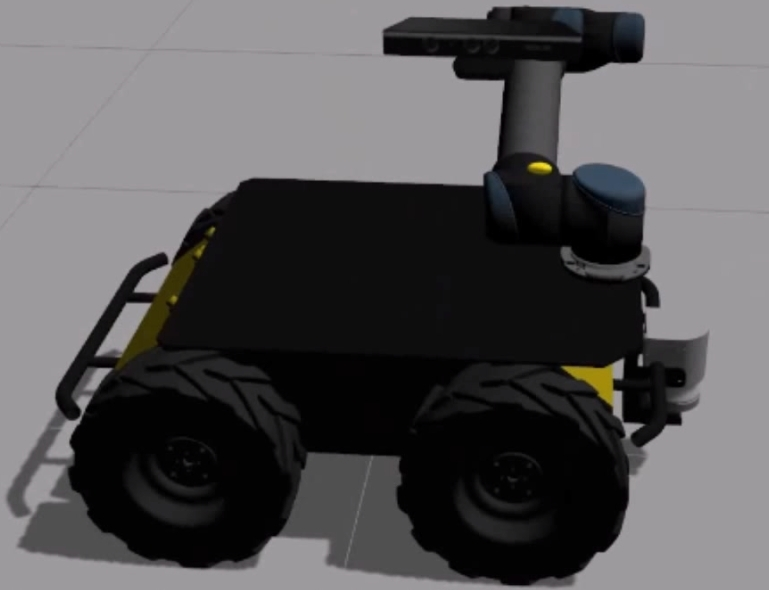
\includegraphics[width=0.5\linewidth]{images/ugv_gazebo_husky.jpg}
  \caption{L'UGV ClearPath Husky avec un modèle de Microsoft Kinect v1 à l'extrémité d'un manipulateur UR5 et un lidar balayeur vers l'avant.}
  \label{fig:ugv_gazebo_husky}
\end{figure}

Le véhicule modélisé est présenté à la Figure \ref{fig:ugv_gazebo_husky} et consiste en un Husky A200 de Clearpath sur lequel un bras manipulater UR5 de Universal Robotics est installé. Bien que le UR5 possède 6 degrés de liberté, nous contraignons son mouvement à 1 seul joint pour respecter la prémisse du problème expliqué dans la section \ref{sec:ugv_problem_description}. L'organe terminal du manipulateur est remplacé par un capteur de profondeur générique aux paramètres de profondeur configurables et la simulation se déroule dans l'environnement de simulation Gazebo. Pour fins d'illustration, l'environnement d'essai est composé d'une structure formée de murets droits. La structure illustrée dans les figures précédentes est dénommée ci-après \guillemotleft Petit $\Gamma$\guillemotright\ et le modèle \guillemotleft Grand $\Gamma$\guillemotright\ est de la même forme, mais aux dimensions deux fois plus grandes. Notre algorithme est aussi comparé à l'algorithme classique l'exploration par frontières proposée par \citep{Yamauchi1997} dans un scénario d'inspection de l'extérieur d'une maison et du modèle Petit $\Gamma$.

\subsubsection{Variation de la taille de structure et de plage de détection profondeur}

Les capteurs de profondeur ont la possibilité de configurer la limite de perception de profondeur ce qui, en plus de la taille de la structure, modifie la trajectoire suivie par l'UGV. Dans toutes les figures, le robot commence sa mission à droite de la structure et bouge initialement vers le bas. Dans la Figure \ref{subfig:small gamma husky 4.5}\ nous pouvons observer le comportement attendu en temps normal de l'algorithme. L'UGV fait un tour de structure pour fermer la boucle pour ensuite entrer dans la cavité. L'inspection se termine lorsque l'UGV ressort de la cavité. Dans la Figure \ref{subfig:small gamma husky 12} la perception est augmentée à 12 mètres. Ici, on ne fait qu'un seul tour de la structure, car quand l'UGV tente de tourner le premier coin, il arrive à percevoir l'intérieur de la cavité. La phase de détection de cavité ne retourne donc rien et la mission se termine. Dans la Figure \ref{subfig:large gamma husky 4.5} le mur de gauche est assez éloigné pour que le détecteur d'obstacles ne se déclenche. Ainsi, l'UGV entre dans la cavité dès la première passe et la mission se termine après un seul tour de la structure. Finalement, la Figure \ref{subfig:large a husky 4.5} démontre un scénario contenant plusieurs cavités et nous pouvons voir que l'algorithme réussit encore à cartographier la structure. Une première passe est réalisée en sautant les cavités et lors de la deuxième passe l'UGV s'arrête en haut à gauche après être sorti de la deuxième cavité. Le Tableau \ref{tbl: simulation results} présente quelques statistiques sur la longueur de trajectoire finale dans les différents scénarios décrits.

\newcommand{\specialcell}[2][c]{%
  \begin{tabular}[#1]{@{}c@{}}#2\end{tabular}}

\begin{table}[ht]
\renewcommand{\arraystretch}{1.3}
\caption{Résultats de simulation pour différentes tailles de la structure et profondeurs de caméra}
\label{tbl: simulation results}
\centering
\begin{tabular}{|c|c|c|c|c|}
\hline
Modèle & \specialcell{Taille du \\périmètre (m)} & \specialcell{Profondeur de\\ la caméra (m)} & \specialcell{Longueur de la \\trajectoire (m)} \\
\hline
Petit $\Gamma$  & $42$ & $4.5$ & $72.08$  \\
Petit $\Gamma$  & $42$ & $12.0$ & $53.79$ \\
Grand $\Gamma$  & $84$ & $4.5$ & $106.23$ \\
Grand \large{a} & $94$ & $4.5$ & $179.65$ \\
\hline
\end{tabular}
\end{table}

\begin{figure}[p]
  \centering
  \subfloat[Modèle: Petit $\Gamma$, Profondeur Max.: $4.5m$]{
      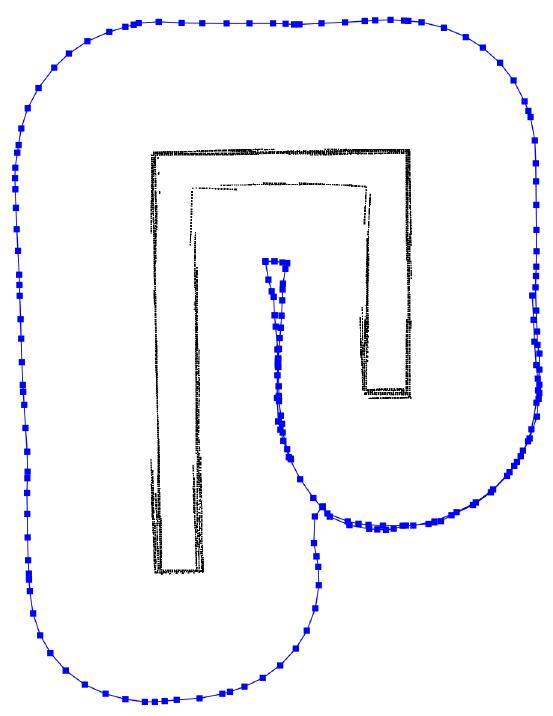
\includegraphics[width=0.4\linewidth]{images/SmallGamma_Husky_4_5}
  	\label{subfig:small gamma husky 4.5}
  }
  \hfil
  \subfloat[Modèle: Petit $\Gamma$, Profondeur Max.: $12m$]{
  	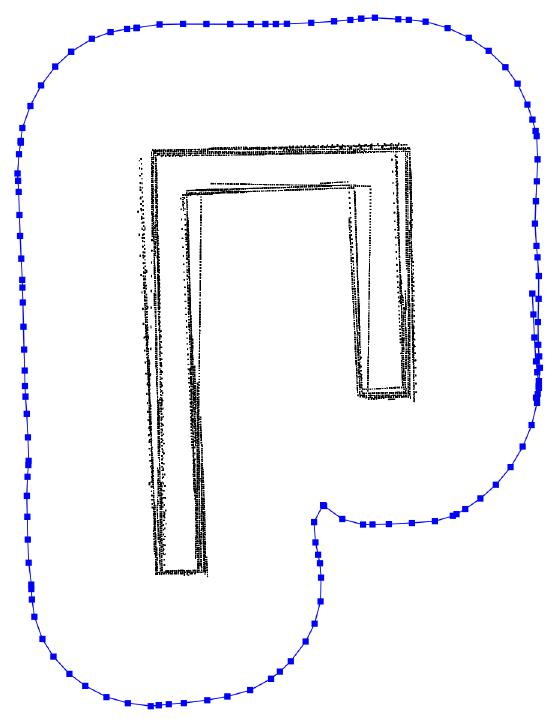
\includegraphics[width=0.4\linewidth]{images/SmallGamma_Husky_12}
  	\label{subfig:small gamma husky 12}
  }
  \hfil
  \subfloat[Modèle: Grand $\Gamma$, Profondeur Max.: $4.5m$]{
  	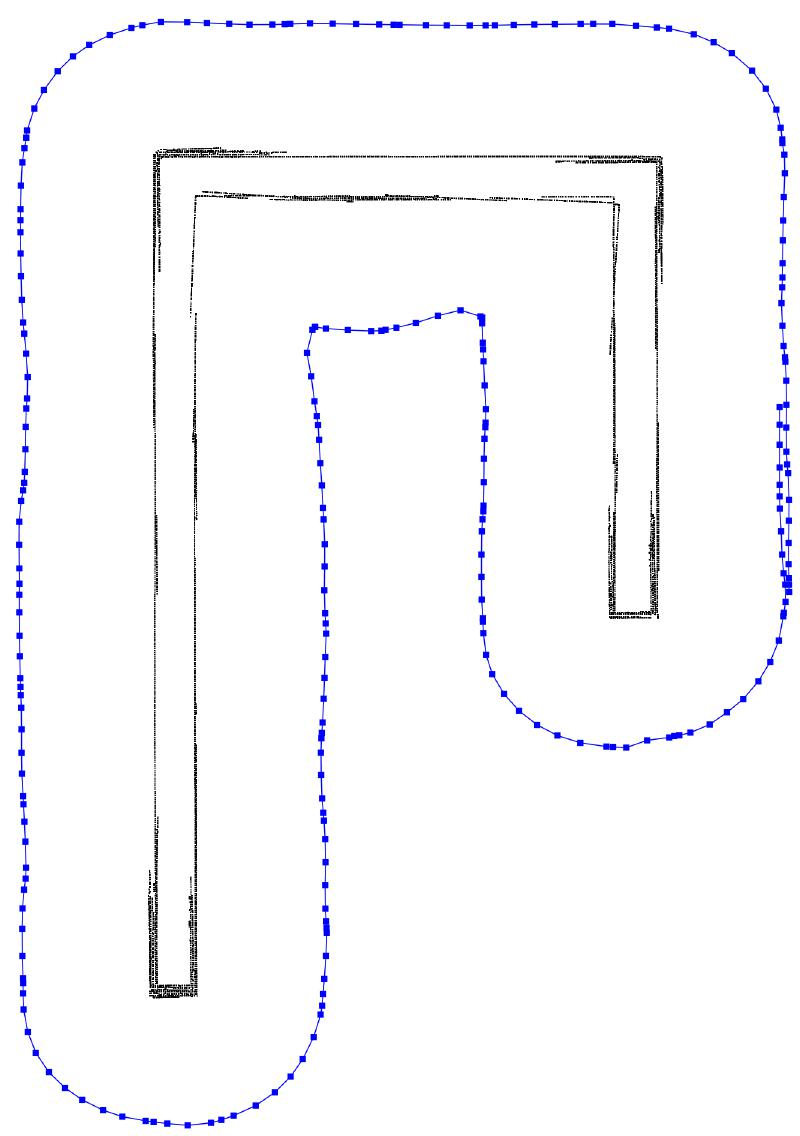
\includegraphics[width=0.4\linewidth]{images/LargeGamma_Husky_4_5}
  	\label{subfig:large gamma husky 4.5}
  }
  \hfil
  \subfloat[Modèle: Grand {\large a}, Profondeur Max.: $4.5m$]{
  	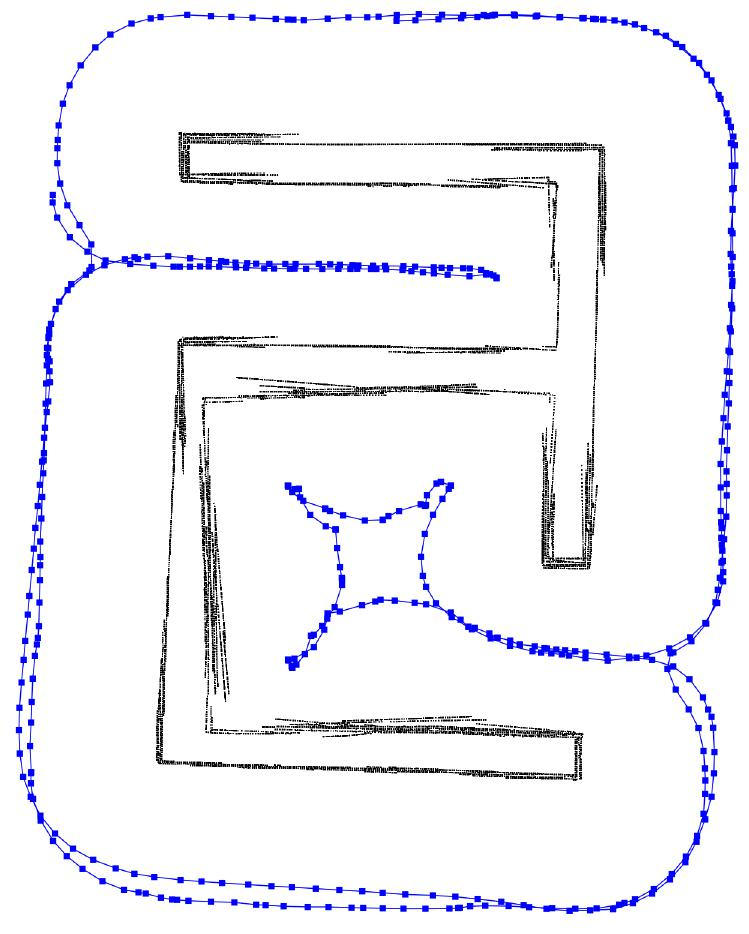
\includegraphics[width=0.4\linewidth]{images/LargeA_Husky_4_5}
  	\label{subfig:large a husky 4.5}
  }
  \caption{
  Projection du modèle reconstruit sur le plan $\vect{x}_{\fr g}\vect{y}_{\fr g}$ en noir et la trajectoire exécutée par le robot en suivant nos algorithmes en bleu.
  }
  \label{fig:relative size}
\end{figure}

\subsubsection{Comparaison à l'exploration par frontier}

Nous comparons notre algorithme à une implémentation de l'exploration par frontière\footnote{\url{http://wiki.ros.org/frontier_exploration}} (EF). L'algorithme prend en entrée les données d'un lidar balayeur 2D pour construire une carte d'occupation sur laquelle les frontières sont calculées. De plus, les bornes d'un polygone 2D délimitant la région à inspecter doivent être fournies. L'inspection se termine lorsqu’aucune frontière n'est trouvé à l'intérieur du polygone. Il existe trois différences majeures entre la solution que nous proposons et l'EF: 1) nous ne requérons pas d'information \textit{a priori} à propos des limites de la région à inspecter; 2) l'EF ne tente pas de se tenir à une distance fixe de la structure pour maximiser la portion de la surface cartographiée; 3) La trajectoire de l'EF est parfois difficile à prévoir comparativement à une stratégie de suivit de mur, ce qui est important d'un point de vue de convivialité. De plus, l'EF peut être affecté par le bruit des capteurs qui cause de légères différences dans la carte d'occupation produite ce qui cause ensuite une génération de trajectoire différente à chaque exécution de l'algorithme. En revanche, notre algorithme produit une trajectoire similaire à chaque exécution. De plus l'EF ne prend pas en compte une distance de sécurité $D$ par rapport à la structure ce qui cause parfois le calcul d'une position objectif très proche de la structure. Ceci est problématique, car, en plus de nuire au capteur de profondeur, l'UGV tend à rester coincé ou en oscillation sur place.

\begin{figure}[p]
  \centering
\subfloat[Notre algorithme]{
	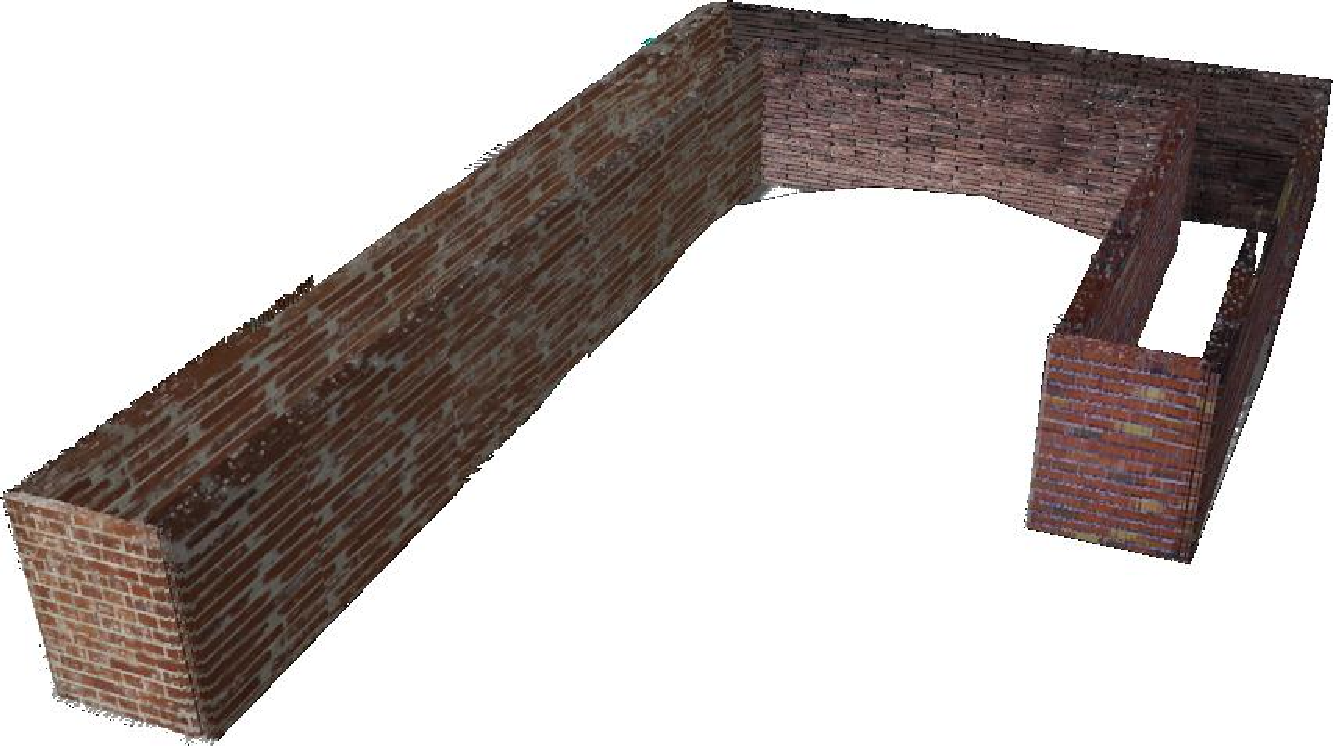
\includegraphics[width=0.3\linewidth]{images/SmallGamma_Husky_4_5_model}
	\label{subfig:small gamma husky 4.5 model}
}
\hfil
\subfloat[Exploration par frontier]{
	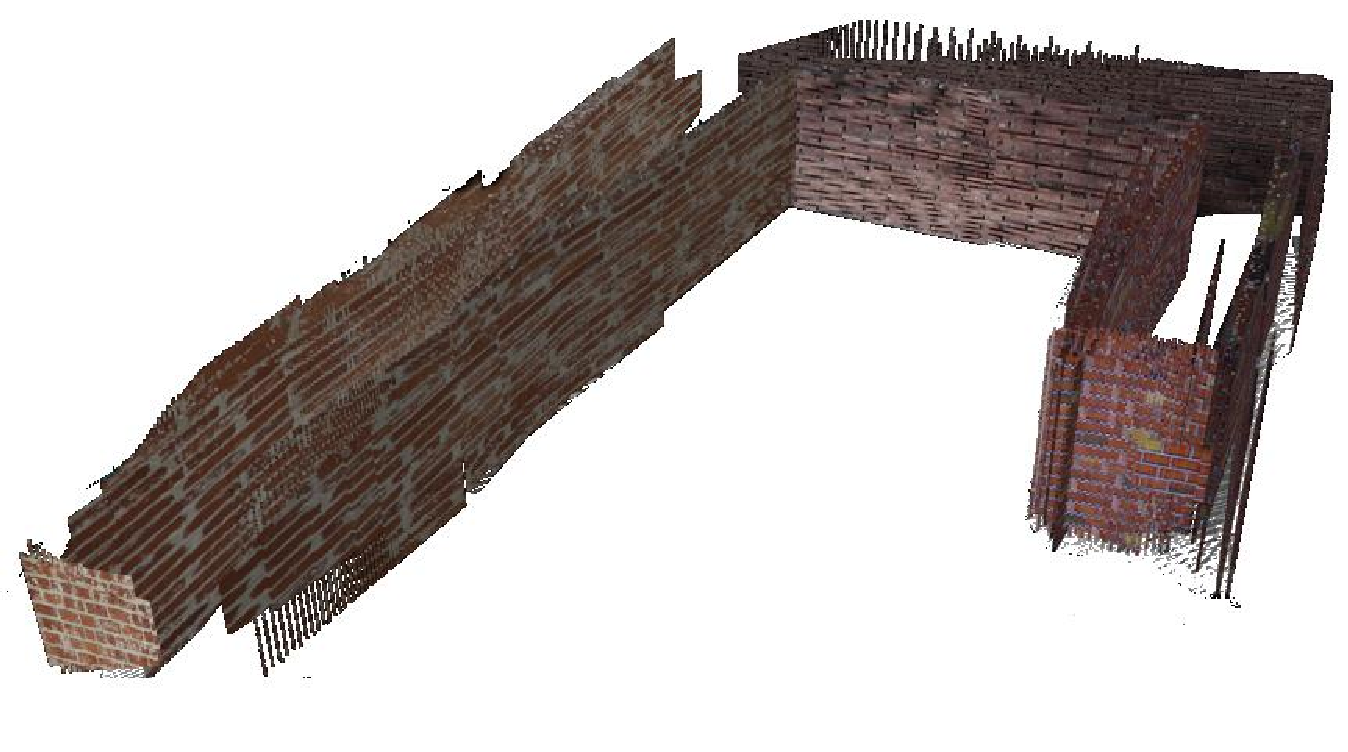
\includegraphics[width=0.3\linewidth]{images/SmallGamma_Husky_4_5_FBE_model}
	\label{subfig:small gamma husky 4.5 FBE model}
}
\hfil
\subfloat[Exploration par frontier]{
	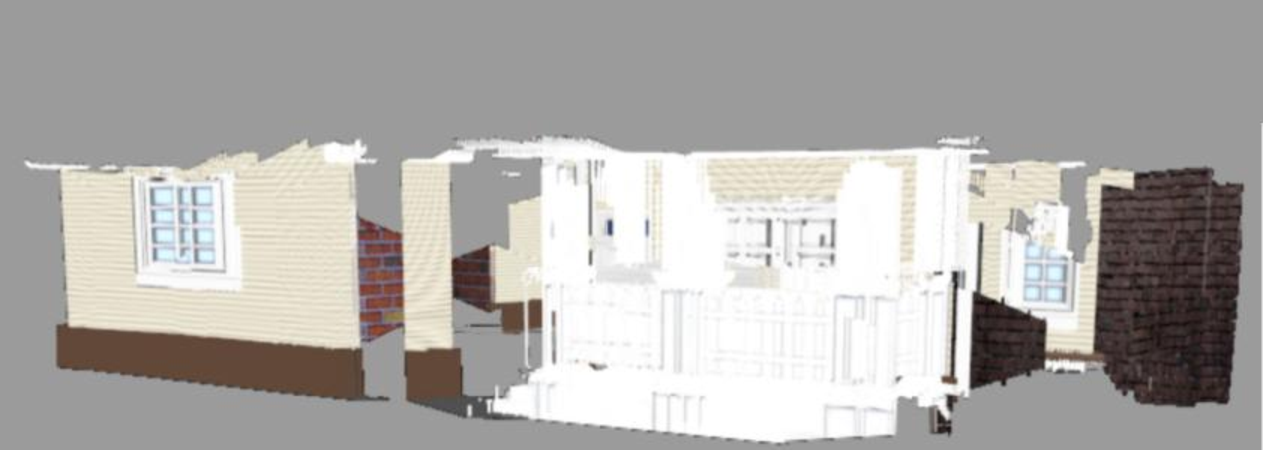
\includegraphics[width=0.8\linewidth]{images/House_FBE_Model}
	\label{subfig:house husky 4.5 FBE model}
}
\hfil
\subfloat[Petit $\Gamma$, Exploration par frontier]{
	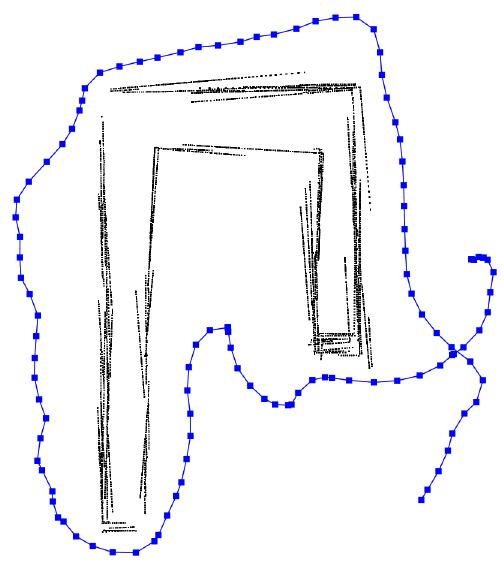
\includegraphics[width=0.3\linewidth]{images/SmallGamma_Husky_FBE_4_5}
	\label{subfig:small gamma husky 4.5 FBE}
}
\hfil
\subfloat[Maison, Exploration par frontier]{
	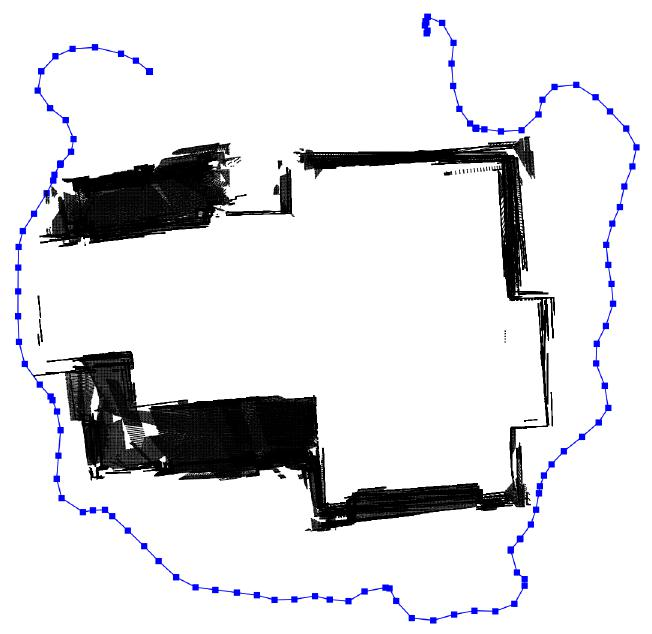
\includegraphics[width=0.3\linewidth]{images/House_Husky_FBE_4_5}
	\label{subfig:house husky 4.5 FBE}
}
\hfil
\caption{ Comparaison entre les résultats de notre algorithme par rapport à l'exploration par frontières avec un capteur de profondeur avec une portée de $4.5\, \mathrm{m}$. On peut voir en (a) par rapport à (B) que l'EF n'assure pas une couverture complète de la surface visible du modèle.
}
\label{fig:simulation FBE}
\end{figure}

Afin de comparer la couverture du modèle, nous utilisons le logiciel CloudCompare pour calculer la projection du modèle reconstruit où $\mathcal C$ est aligné au modèle de référence discrétisé $\mathcal C_R$. Pour les deux modèles Petit $\Gamma$ et celui de la maison, la discrétisation se fait avec un distance minimale de $0.1$m entre chaque point et seulement sur la portion allant jusqu'à la hauteur maximale perceptible $H_{max}$. Pour l'alignement de $\mathcal C$  à $\mathcal C_R$, une procédure de \textit{iterative closest point} (ICP) \citep{Rusinkiewicz2001} a été utilisée. Ensuite, pour chaque point de $\mathcal C$, on recherche le point de référence le plus proche dans $\mathcal C_R$. Dans le cas où un point de $\mathcal C_R$ est associé à plusieurs points de $\mathcal C$, nous enlevons les points dupliqués pour obtenir l'ensemble des points uniques les plus proches de la structure. Le nombre de points dans cet ensemble devient notre métrique par laquelle nous estimons la couverture du modèle. Finalement, nous calculons aussi l'erreur moyenne qui correspond à la distance moyenne entre les points de l'ensemble unique et ceux du modèle.

Le Tableau \ref{tbl: simulation results 3} montre la différence entre notre stratégie et l'EF avec une caméra de profondeur limitée à $4.5\, \mathrm{m}$. En somme, notre algorithme réussit systématiquement à obtenir une couverture plus élevée en plus d'une trajectoire plus courte. De plus, nous notons que la trajectoire lisse gardant toujours en vue la structure permet d'obtenir une erreur de reconstruction plus petite. De plus, la Figure \ref{fig:simulation FBE} démontre qualitativement l'amélioration en termes des couvertures de notre algorithme et les lacunes au niveau de la reconstruction de l'EF.

\begin{table}[!ht]
\renewcommand{\arraystretch}{1.3}
\caption{Comparaison entre notre algorithme et l'EF}
\label{tbl: simulation results 3}
\centering
\begin{tabular}{|c|c|c|c|}
\cline{3-4}
\multicolumn{2}{c|}{} & Notre algorithme & EF \\
\hline
{Petit $\Gamma$} & Trajectoire (m)            & $72.08$  & $49.78$  \\\cline{2-4}
								& \specialcell{\# de points uniques les plus proches \\ (maximum de 6116)} & $6,063$          & $5,398$          \\\cline{2-4}
								& Erreure moyenne (m)             & $0.05$ & $0.12$\\\cline{2-4}
\hline
{Maison} & Trajectoire (m) & $59.89$ & $47.55$ \\\cline{2-4}
					   & \specialcell{\# de points uniques les plus proches \\ (maximum de 10 889)} & $9,182$ & $7,402$ \\\cline{2-4}
					   &  Erreure moyenne (m)             & $0.05$ & $0.12$\\\cline{2-4}
\hline
\end{tabular}
\end{table}


\subsection{Résultats expérimentaux}

L'implémentation sur un vrai robot a été réalisée sous des conditions similaires à la simulation où un Husky est équipé d'un bras robotique Kinova Mico au bout duquel un capteur de profondeur Microsoft Kinect v2 est attaché. En guise de détecteur d'obstacle, un scanner lidar SICK LMS511 est installé à l'avant. Contrairement à nos simulations, nous effectuons nos tests dans un environnement intérieur dépourvu de signal GPS. C'est pourquoi ici l'odométrie provient de la fusion de seulement l'odométrie des roues et de la centrale inertielle dans l'EKF de \citep{MooreEkf2014}. Cette odométrie est ensuite envoyée à RTAB-Map \citep{Labbe2014} pour fins de localisation et de cartographie. L'intégralité des calculs se déroule sur un ordinateur à base d'un processeur Intel i5 sans l'aide d'un GPU. La structure à inspecter imite le modèle Petit $\Gamma$ avec les dimensions de $8.2\text{ m} \times 4\text{ m}$ et a été construite avec un mélange de panneaux d'isolation et des panneaux de liège amovibles. Pour assurer une fermeture de boucle, nous plaçons une pancarte colorée à l'endroit de départ du UGV visible dans les Figures \ref{fig:husky_exp_structure} et \ref{subfig:loop_closure_success}. Nous voyons clairement la différence entre la situation \ref{subfig:fail_loop_closure} où la mise en correspondance échoue et la situation en \ref{subfig:loop_closure_success} où les caractéristiques uniques de notre pancarte aide le système de SLAM.

Puisque l'espace dans notre aire de test était limité, nous réduisons la portée de notre détecteur d'obstacles à $1.8\, \mathrm{m}$ et à un cône de $10^\circ$  en avant du Husky. La profondeur de la caméra a été limitée à $4.0\, \mathrm{m}$ et nous configurons la distance au mur $D=1.5\, \mathrm{m}$. De plus, puisque nous savons que l'UGV ne bouge pas en $\vect{z}^g$ et que nous supposons que le terrain est plat, nous contraignons RTAB-Map à $3$ degrés de liberté ($\vect{x}^g$, $\vect{y}^g$ et l'angle de lacet $\psi$).

\begin{figure}[htb]
\centerline{
	\subfloat[]{
		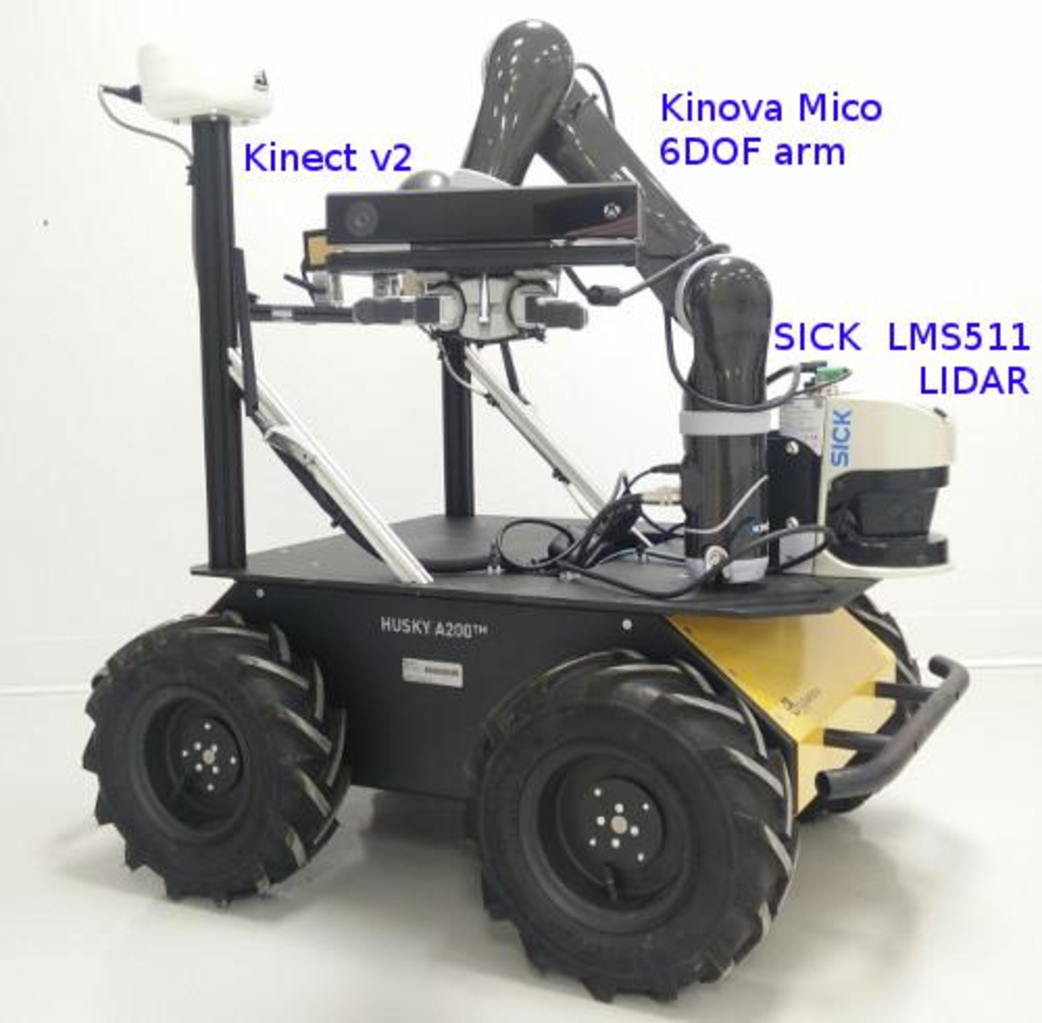
\includegraphics[width=0.43\linewidth]{images/husky_annotated.pdf}
        \label{fig:husky_exp_sensors}
    }%
    \subfloat[]{
		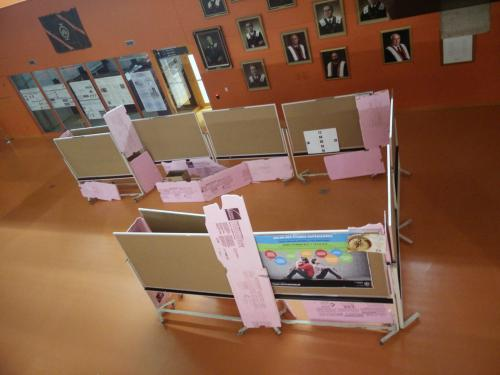
\includegraphics[width=0.57\linewidth]{images/structure.pdf}
        \label{fig:husky_exp_structure}
	}
}
	\centering
    \caption{
    (a) Le robot Husky utilisé dans nos expériences avec le bras articulé, le capteur de profondeur et le scanner lidar. Les autres capteurs non identifiés ne sont pas utilisés dans lors de l'expérience.
    (b) La structure intérieure sous inspection.}
    \label{fig:husky_exp}
\end{figure}

\begin{figure}[ht]
  \centering
  \subfloat[]{
  	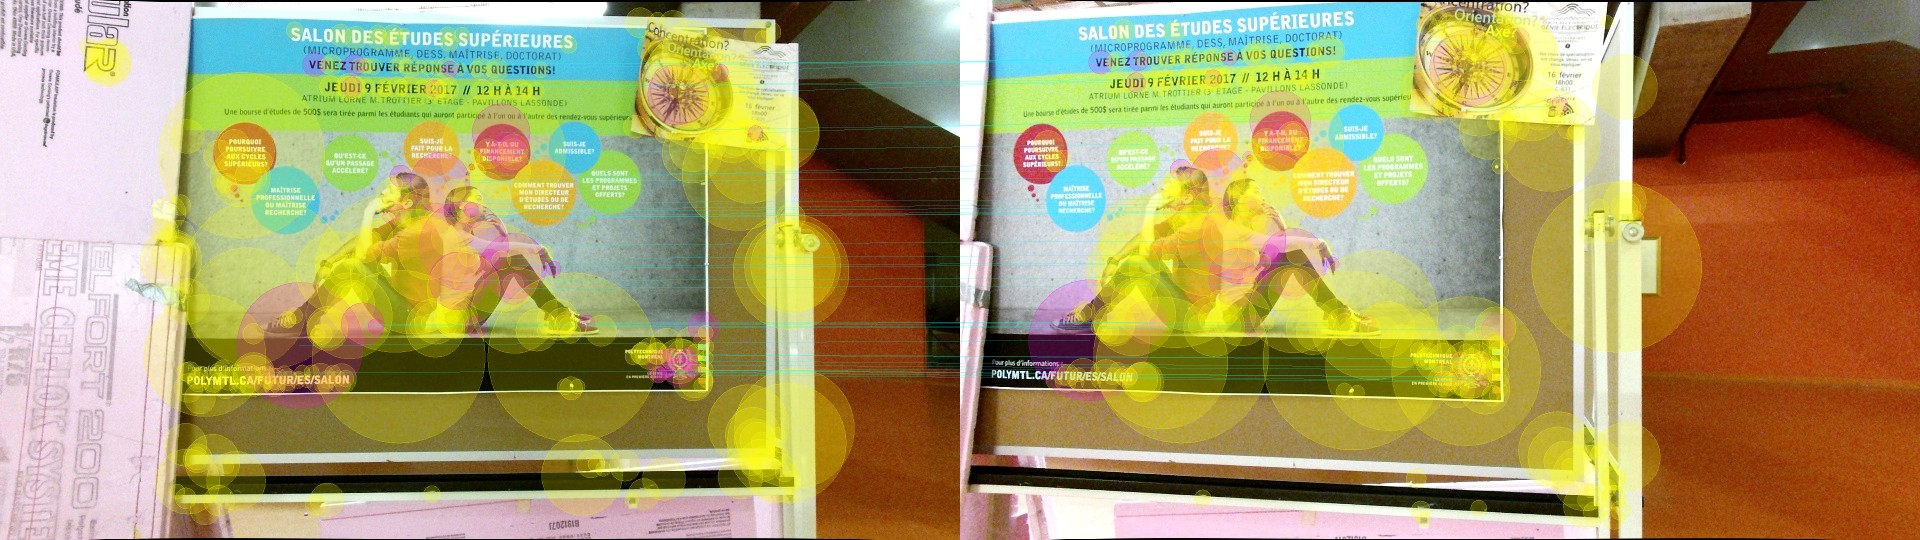
\includegraphics[width=0.8\linewidth]{images/loop_closure_vslam.jpg}
  	\label{subfig:loop_closure_success}
  }
  \hfil
  \subfloat[]{
  	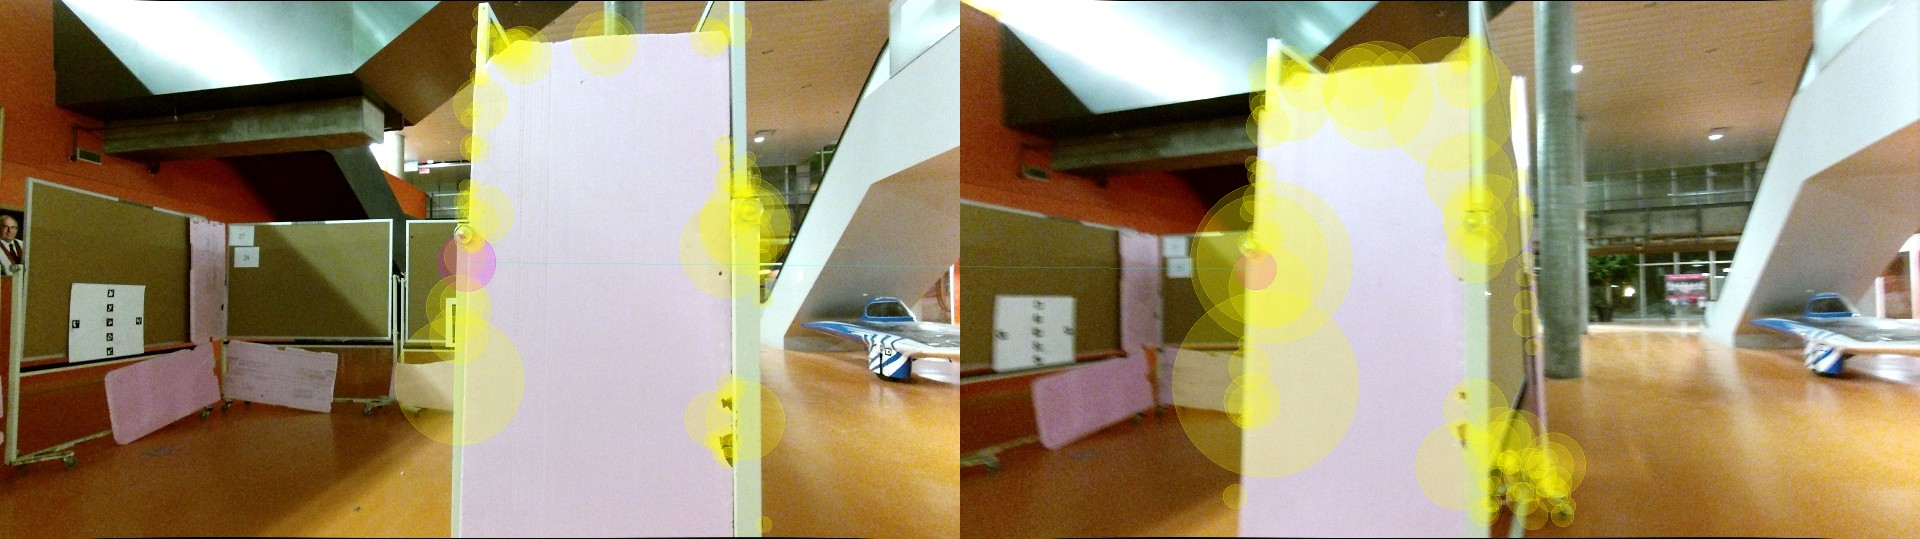
\includegraphics[width=0.8\linewidth]{images/loop_closure_fail}
  	\label{subfig:fail_loop_closure}
  }
  \caption{
    Tentatives de fermetures de boucle du système de SLAM RTAB-Map. Les lignes cyan représentent des mises en correspondances de caractéristiques entre l'image de référence (gauche) et l'image courante (droite).
    (a) Succès de la fermeture de boucle avec plusieurs mises en correspondances. (b) Tentative échouée de fermeture de boucle avec qu'une seule mise en correspondance.
  }
  \label{fig:visual_loop_closure}
\end{figure}

Le comportement de notre algorithme est illustré dans la Figure \ref{fig:exp_angled_view} et reflète presque le comportement prédit dans la simulation. Rappelons que pour une cavité, l'algorithme de détection d'entrée retournera typiquement deux entrées de part et d'autre de l'ouverture dans la structure. En temps normal, la deuxième entrée sera enlevée de la liste des candidats lorsque son centroïde entrera en vue de la caméra de profondeur à la sortie de la cavité. Il semblerait que lors de l'expérience, la détection du centroïde a échoué, car l'UGV s'est retrouvé entre la structure et le centroïde à détecter. Ceci cause l'UGV à effectuer un deuxième tour autour de la structure avant de s'arrêter près de l'entrée. Nous voyons donc que si une partie de l'algorithme échoue, dans le pire cas le robot effectue simplement un deuxième tour.

\begin{figure}[!ht]
  \centering
  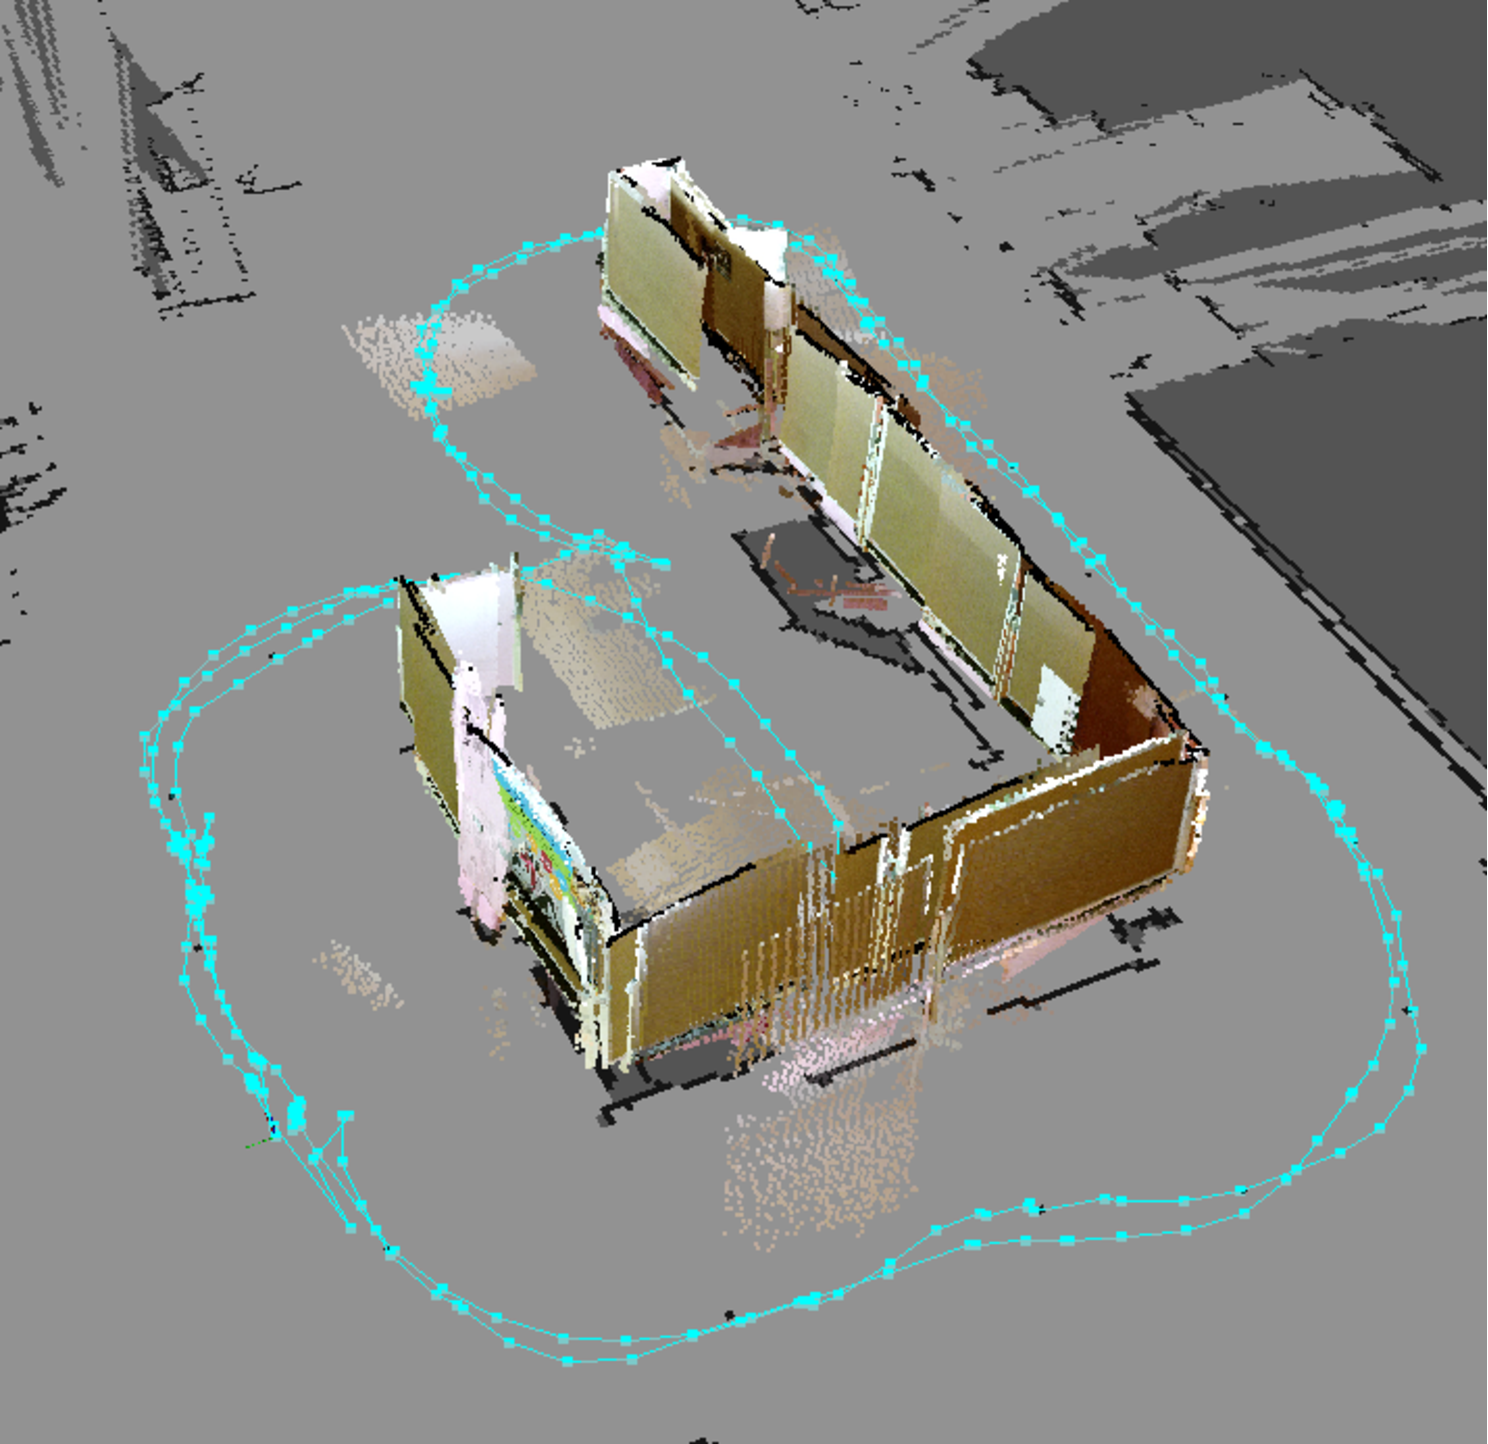
\includegraphics[width=0.5\linewidth]{images/exp_angled_view}
  \caption{Résultat expérimental, en cyan la trajectoire, en gris la carte d'occupation et d'obstacles créée par l'assemblage des balayages du lidar et en couleur la reconstruction du modèle par nuage de points.}
  \label{fig:exp_angled_view}
\end{figure}

\subsubsection{Performance à l'exécution}

Le robot réussit à faire l'exploration du périmètre en sautant la cavité interne, le tout en temps réel malgré l'exécution du SLAM 3D et des différents algorithmes d'estimation d'odométrie et de planification de trajectoire. La partie la plus lente de l'algorithme reste la construction et l'analyse de l'OctoMap pour la détection des cavités qui peut prendre plusieurs secondes de temps. Bien que la représentation multi résolution d'un OcTree nous permet d'accélérer les requêtes à la carte, un problème existe néanmoins dans l'insertion des points et du traçage des rayons associés qui se fait séquentiellement sans l'utilisation de fils d'exécution en parallèle. Ceci pourrait être réglé en changeant la représentation utilisée d'OctoMap à une représentation parallélisable tel que la SkiMap récemment proposé par \citep{Gregorio2017}.

\subsection{Sources de bruit et différences entre la simulation et l'expérience réelle}
\label{subsec:ugv_noise_sim}

En effectuant nos expériences, nous notons plusieurs différences entre notre environnement de simulation et la réalité. La première que nous remarquons est la quantité de bruit dans les capteurs. Dans notre environnement Gazebo, la caméra de profondeur est simulée avec un bruit gaussien sur les mesures de distances et chaque pixel de l'image de profondeur est en fait simulé par les mêmes mécanismes de simulation de laser. En réalité, les capteurs fonctionnant par ToF possèdent des caractéristiques de bruit légèrement différentes, entre autres, du bruit poivre et sel, et du bruit de chatoiement (des petites taches dans l'image). Cette dernière est particulièrement importante, car elle peut facilement faire échouer le calcul de la prochaine pose objectif tel que présenté dans la Figure \ref{fig:speckle_fail}.

\begin{figure}[!th]
  \centering
  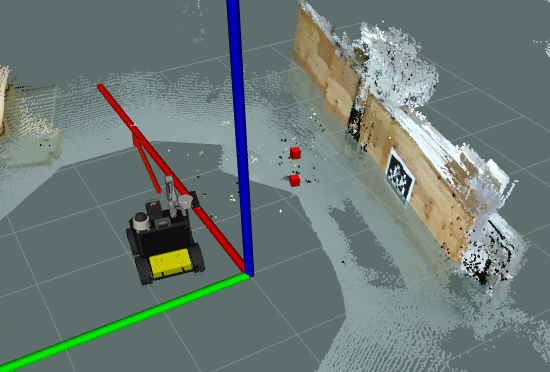
\includegraphics[width=0.7\linewidth]{images/speckle.png}
  \caption{Échec du suivit de la structure par la présence de bruit de chatoiement. Les cubes rouges sont en fait des taches qui ont étés considérées comme une partie de la structure alors qu'en réalité elles n'existent pas.}
  \label{fig:speckle_fail}
\end{figure}

En traitement d'images, le bruit poivre et sel serait normalement éliminé par un filtre médian \citep{jayaraman2009digital}. Par contre, puisque nous voulons utiliser les images de profondeur pour la reconstruction et la navigation de notre robot, nous voulons préserver autant que possible les détails originaux des données. Le bruit poivre et sel est donc éliminé simplement par seuillage en imposant une limite supérieure et inférieure sur les distances perçues. Tout point en dehors de la plage acceptable n'est pas projeté dans le nuage de points utilisé pour la navigation et la cartographie. Pour cette même raison, nous n'appliquons pas de filtre bilatéral sur l'image de profondeur pour éliminer le bruit de chatoiement, car ce filtre pourrait lisser les contours de certains obstacles. À la place, nous appliquons un filtre de déchatoiement qui cherche des groupes de pixels connectés et qui impose ensuite une taille minimale sur ces groupes. Ceci est fait directement sur l'image de profondeur avant la projection à un nuage de points. Pour calibrer les paramètres du filtre, nous plaçons l'UGV à l'endroit où le plus de bruit est détecté et nous augmentons progressivement la taille maximale des taches à enlever jusqu'à ce que l'image de profondeur soit libre de bruit. Il faut aussi calibrer la différence maximale entre deux pixels pour les considérer dans le même groupe. Ce dernier paramètre peut être deviné intuitivement puis raffiné expérimentalement en inspectant une scène contenant plusieurs objets à diverses distances.

Outre le bruit de capteur, certaines différences inattendues se sont présentées physiquement sur le robot, causant une dégradation de la performance de cartographie. Premièrement, en raison de la taille des panneaux et de la distance limitée autour de la structure, le bras Kinova a été étendu à une hauteur de $1.2\, \mathrm{m}$ causant ainsi des vibrations sur caméra de profondeur et des images floues envoyées au système de SLAM. La fermeture de boucle échoue parfois en raison d'une mauvaise extraction des caractéristiques de l'image. Ce problème pourrait être mitigé de plusieurs façons: en utilisant un meilleur contrôle sur l'accélération maximale du robot, en installant le capteur sur une plateforme orientable plus rigide et en opérant dans un environnement mieux illuminé pour réduire le temps d'exposition du capteur RGB. Deuxièmement, le modèle Petit $\Gamma$ utilisé en simulation était assemblé de plusieurs prismes rectangulaires créant ainsi une structure parfaitement lisse. Par contre, dans notre assemblage de panneaux de liège, il existait plusieurs trous et ouvertures dans la structure auxquels l'algorithme \ref{alg:PE_next_goal} pour le suivi de mur est sensible. En effet, lorsqu'elle est devant une fenêtre, la caméra de profondeur tend à capter des surfaces à l'intérieur de la structure affectant ainsi le calcul de la normale de la surface. Pour mitiger ce problème, il est utile de limiter la portée du capteur de profondeur à une valeur légèrement au-dessus de la distance au mur $D$.

En somme, notre algorithme est surtout sujet à deux sortes de cas d'échec: i) l'échec du calcul de la trajectoire d'inspection par la présence de trous et de fenêtres dans la structure et ii) l'échec de la fermeture de boucle globale que nous pouvons mitiger à l'aide d'un marqueur visuel unique.

\section{Conclusion} \label{sec:ugv_conclusion}

En conclusion, nous avons présenté une méthode pour la génération de trajectoire permettant de guider un UGV équipé d'une caméra de profondeur mobile pour l'inspection d'une structure fermée inconnue. Notre méthode ne requiert aucune information \textit{a priori} sur la taille ou sur la géométrie de la structure. Utilisé en conjonction avec un système de SLAM visuel performant, nous obtenons une grande couverture de la surface de la structure dans le modèle reconstruit malgré les limites de la plateforme. Le système proposé est validé en simulation et dans des tests expérimentaux. Par une comparaison à l'algorithme classique d'exploration par frontières, nous démontrons clairement le gain en performance dans le cas d'une structure réaliste telle qu'une maison.

Finalement, la méthode proposée garantie que le robot parcourt l'entièreté du périmètre de la structure, mais elle ne garantit pas que l'entièreté de la surface sera cartographiée. Pour ce faire, nous pourrions ajouter un planificateur de trajectoire secondaire pour déplacer la caméra localement au moyen du bras articulé pour assurer une couverture complète à chaque point d'inspection. De plus, il reste plusieurs améliorations possibles à apporter à l'algorithme, notamment l'utilisation d'une représentation autre que l'OctoMap telle que AtomMap, SkiMap ou les TSDF ou du moins la parallélisation du calcul des entrées de cavité. D'un autre côté, nous pourrions profiter du bras articulé pour ajouter des degrés de liberté à la caméra de profondeur. Ceci permettrait de faire une planification de trajectoire secondaire pour optimiser davantage le positionnement de la caméra ou même de faire une planification de trajectoire globale prenant en compte les possibilités additionnelles.
